%%
%% This is file `sample-xelatex.tex',
%% generated with the docstrip utility.
%%
%% The original source files were:
%%
%% samples.dtx  (with options: `sigconf')
%% 
%% IMPORTANT NOTICE:
%% 
%% For the copyright see the source file.
%% 
%% Any modified versions of this file must be renamed
%% with new filenames distinct from sample-xelatex.tex.
%% 
%% For distribution of the original source see the terms
%% for copying and modification in the file samples.dtx.
%% 
%% This generated file may be distributed as long as the
%% original source files, as listed above, are part of the
%% same distribution. (The sources need not necessarily be
%% in the same archive or directory.)
%%
%%
%% Commands for TeXCount
%TC:macro \cite [option:text,text]
%TC:macro \citep [option:text,text]
%TC:macro \citet [option:text,text]
%TC:envir table 0 1
%TC:envir table* 0 1
%TC:envir tabular [ignore] word
%TC:envir displaymath 0 word
%TC:envir math 0 word
%TC:envir comment 0 0
%%
%%
%% The first command in your LaTeX source must be the \documentclass
%% command.
%%
%% For submission and review of your manuscript please change the
%% command to \documentclass[manuscript, screen, review]{acmart}.
%%
%% When submitting camera ready or to TAPS, please change the command
%% to \documentclass[sigconf]{acmart} or whichever template is required
%% for your publication.
%%
%%
\documentclass[sigconf,nonacm]{acmart}

%%
%% \BibTeX command to typeset BibTeX logo in the docs
%\AtBeginDocument{%
%  \providecommand\BibTeX{{%
%    Bib\TeX}}}
%
%%% Rights management information.  This information is sent to you
%%% when you complete the rights form.  These commands have SAMPLE
%%% values in them; it is your responsibility as an author to replace
%%% the commands and values with those provided to you when you
%%% complete the rights form.
%\setcopyright{acmcopyright}
%\copyrightyear{2018}
%\acmYear{2018}
%\acmDOI{XXXXXXX.XXXXXXX}
%
%%% These commands are for a PROCEEDINGS abstract or paper.
%\acmConference[Conference acronym 'XX]{Make sure to enter the correct
%  conference title from your rights confirmation emai}{June 03--05,
%  2018}{Woodstock, NY}
%%%
%%%  Uncomment \acmBooktitle if the title of the proceedings is different
%%%  from ``Proceedings of ...''!
%%%
%%%\acmBooktitle{Woodstock '18: ACM Symposium on Neural Gaze Detection,
%%%  June 03--05, 2018, Woodstock, NY}
%\acmPrice{15.00}
%\acmISBN{978-1-4503-XXXX-X/18/06}


%%
%% Submission ID.
%% Use this when submitting an article to a sponsored event. You'll
%% receive a unique submission ID from the organizers
%% of the event, and this ID should be used as the parameter to this command.
%%\acmSubmissionID{123-A56-BU3}

%%
%% For managing citations, it is recommended to use bibliography
%% files in BibTeX format.
%%
%% You can then either use BibTeX with the ACM-Reference-Format style,
%% or BibLaTeX with the acmnumeric or acmauthoryear sytles, that include
%% support for advanced citation of software artefact from the
%% biblatex-software package, also separately available on CTAN.
%%
%% Look at the sample-*-biblatex.tex files for templates showcasing
%% the biblatex styles.
%%

%%
%% The majority of ACM publications use numbered citations and
%% references.  The command \citestyle{authoryear} switches to the
%% "author year" style.
%%
%% If you are preparing content for an event
%% sponsored by ACM SIGGRAPH, you must use the "author year" style of
%% citations and references.
%% Uncommenting
%% the next command will enable that style.
%%\citestyle{acmauthoryear}


\usepackage{pifont}
\usepackage{url}
\usepackage{subfigure}
\usepackage[ruled]{algorithm2e}
\usepackage{algorithmic}
\usepackage{bbding}

%%
%% end of the preamble, start of the body of the document source.
\begin{document}

%%
%% The "title" command has an optional parameter,
%% allowing the author to define a "short title" to be used in page headers.
\title{GSnap: An Efficient Group-based Snapshot Index in the Cloud Database}

%%
%% The "author" command and its associated commands are used to define
%% the authors and their affiliations.
%% Of note is the shared affiliation of the first two authors, and the
%% "authornote" and "authornotemark" commands
%% used to denote shared contribution to the research.
% \author{Xiaoshuang Peng$^1$, Xiaopeng Fan$^1$, Chuliang
%	Weng$^1$$^\ast$, Shi Cheng$^2$, Lingbin Meng$^2$, Cuiyun
%	Fu$^2$, and Feifei Li$^2$} \affiliation{% \institution{ East
%	China Normal University$^1$, Alibaba Group$^2$ } }
%%\email{{xspeng, xpfan}@stu.ecnu.edu.cn, clweng@dase.ecnu.edu.cn, 
%%	{chengshi.cs, lingbin.mlb, cuiyun.fcy, lifeifei}alibaba-inc.com}
%\email{{xspeng, xpfan}@stu.ecnu.edu.cn, clweng@dase.ecnu.edu.cn,}
%
%\email{{chengshi.cs, lingbin.mlb, cuiyun.fcy, lifeifei}@alibaba-inc.com}

\author{XXX}

%%
%% By default, the full list of authors will be used in the page
%% headers. Often, this list is too long, and will overlap
%% other information printed in the page headers. This command allows
%% the author to define a more concise list
%% of authors' names for this purpose.
%\renewcommand{\shortauthors}{Trovato et al.}

%%
%% The abstract is a short summary of the work to be presented in the
%% article.
\begin{abstract}
		Database often takes full and incremental snapshots of
                its fine-grained status, to support database
                recovery. In recent years, cloud native database and
                data warehouse tend to query those snapshots using
                time travel for instant recovery, flashback, and data
                tracking. This requires the system to efficiently
                query large scale data blocks across continuous
                snapshots. However, existing snapshot technologies do
                not meet the requirement. The write amplification of
                Copy-on-Write (CoW) introduces additional expensive
                I/O operations, which severely degrade performance. In
                the Redirect-on-Write (RoW) which is more widely used
                in cloud storage, the updated data blocks are
                scattered among the snapshots, resulting in a
                dependency between the snapshots. This dependency
                introduces significant overhead for queries on the
                snapshots.

                In this paper, we observe that the access of snapshots
                has strong locality and continuity. We therefore
                propose an efficient RoW-based snapshot index, called
                GSnap, which groups snapshot indexes based on cloud
                database workload and access behavior of
                snapshot. Specifically, we use two key techniques:
                Shared-Subtrees Indexing (SSI) and Group-Based
                Dividing (GBD), to perform split dependency of the
                snapshot index.  In-group snapshot indexes reduce
                memory overhead by sharing subtrees. The snapshot
                index dependency chain is divided into groups and
                there is no dependency on snapshot indexes between
                groups.  The index can directly locate data blocks
                instead of iterative traversal.  At the same time, the
                design of the snapshot index deletion method is
                adapted to the snapshot sparse deletion model.  We
                have implemented a prototype system in Ceph.
                Evaluation results with datasets demonstrate that,
                compared with state-of-the-art techniques, GSnap could
                effectively balance the overhead between index memory
                usage and recovery time.
\end{abstract}

%%
%% The code below is generated by the tool at http://dl.acm.org/ccs.cfm.
%% Please copy and paste the code instead of the example below.
%%
%\begin{CCSXML}
%<ccs2012>
% <concept>
%  <concept_id>10010520.10010553.10010562</concept_id>
%  <concept_desc>Computer systems organization~Embedded systems</concept_desc>
%  <concept_significance>500</concept_significance>
% </concept>
% <concept>
%  <concept_id>10010520.10010575.10010755</concept_id>
%  <concept_desc>Computer systems organization~Redundancy</concept_desc>
%  <concept_significance>300</concept_significance>
% </concept>
% <concept>
%  <concept_id>10010520.10010553.10010554</concept_id>
%  <concept_desc>Computer systems organization~Robotics</concept_desc>
%  <concept_significance>100</concept_significance>
% </concept>
% <concept>
%  <concept_id>10003033.10003083.10003095</concept_id>
%  <concept_desc>Networks~Network reliability</concept_desc>
%  <concept_significance>100</concept_significance>
% </concept>
%</ccs2012>
%\end{CCSXML}
%
%\ccsdesc[500]{Computer systems organization~Embedded systems}
%\ccsdesc[300]{Computer systems organization~Redundancy}
%\ccsdesc{Computer systems organization~Robotics}
%\ccsdesc[100]{Networks~Network reliability}

%%
%% Keywords. The author(s) should pick words that accurately describe
%% the work being presented. Separate the keywords with commas.
\keywords{cloud native database, snapshot, database recovery, time travel}
%% A "teaser" image appears between the author and affiliation
%% information and the body of the document, and typically spans the
%% page.



%%
%% This command processes the author and affiliation and title
%% information and builds the first part of the formatted document.
\maketitle

\section{Introduction}
Databases perform full and incremental backup to ensure data
reliability and durability, and provide point-in-time recovery (PITR)
capability for protection against accidental deletion or
writes. Modern database backup copies \cite{rubirk, cohesity} are not
saved in a separate location from original data.  Backup clones
immutable snapshot into writable volume and live mounts to do instant
recovery, which is called Cloud Data Management (CDM)
\cite{zhao2014cloud}.

Cloud native databases can fully take the advantages of cloud storage
to provide hundreds of thousands snapshots. Part of the snapshots are
stored in the Cloud Block Storage (CBS) whereas the rest of snapshots
are archived to the Cloud Object Storage (COS) to support more
snapshots and reduce their cost. The snapshots in CBS can be instantly
cloned and mounted while archived snapshots in COS normally need to be
copied to CBS for recovery.  The snapshot could even be taken once
every 10 minutes in Google Cloud Persistent disk\cite{GoolgeCloudPDS},
and the number of snapshots per volume is up to 5000 in Rackspace
Cloud Block Storage \cite{RackspaceCloudblockstorage}.  Cloud vendors
support a single snapshot instantly restore and flashblack. For
example, AWS EBS \cite{varia2014overview} provides Fast Snapshot
Restore (FSR) to accelerate volume creation from the snapshot and
eliminates the latency of I/O operations on a block when it is
accessed for the first time. Azure Backup \cite{Azurebackup} improves
restore performance with Instant Restore capability for VM
snapshot. On Alibaba Cloud, PolarDB \cite{polardb} and RDS \cite{AliyunRDS}
provide similar instant recovery capacity and features like flashback.


Considerable number of snapshots leads to a new trend that databases
always separate business and data track on multiple snapshots.  For
example, MongoDB supports row-level query on the queryable snapshots,
which are similar to the read-only MongoDB instances. Data warehouse
such as Snowflake \cite{snowflake}, AnalyticDB \cite{AnalyticDBMySQL}
and Delta Lake \cite{Deltalake} also provide time travel capability on
continuous snapshots to access historical data at any point within a
specified time period. Besides, the declarative extensions
\cite{tsikoudis2020rid,tsikoudis2018rql,shrira2005snap} to SQL are
developed to specify and run multi-snapshot computations conveniently
for auditing and other forms of fact checking.  The new trend has a
continuous access feature instead of accessing just a single snapshot,
and is similarly sensitive to instant recovery latency. Real-time
queries also need to be supported.


However, existing snapshot technologies do not meet the requirements.
%	The snapshot only stores data blocks that have been modified
%	during the process of taking the snapshot, which could greatly
%	decrease storage overhead.
For Copy-on-Write (CoW)
\cite{nightingale2008rethink,chidambaram2013optimistic}, it introduces
write amplification because the data blocks are copied to the
snapshot, then the new data is written to the data blocks on the
device.  It is unacceptable for cloud providers that the write
amplification problem severely degrades performance
\cite{merenstein2021cnsbench}. Thus, an alternative strategy is
Redirect-on-Write (RoW).  For RoW, the updated data blocks are
scattered while the unupdated data blocks point to the previous
snapshots. Restoring a snapshot requires access to several
snapshots. Thus more additional snapshots need to be accessed if
restore continuous snapshots, which increases the recovery latency and
degrades the query performance of the snapshots.

%The length of the snapshot set is determined by the query
%date. Besides, they may combine multiple snapshot sets for
%cross-querying.

Snapshot recovery includes index and data block recovery, which are
both stored in the remote storage system. The snapshot builds indexes
and then loads data blocks. Index recovery includes loading index from
the remote node and locating the address of the data block locally. In
RoW, index recovery needs to load more indexes because of the
dependency, and the number of hops in locating is linearly related to
the number of snapshots. Large index size increases recovery latency
and memory overhead, which may saturate network bandwidth and
computing resource of the storage system.  Many works tend to build
data block indexes
\cite{yang2011st,joseph2019securing,pekerskaya2006mining} to
accelerate the recovery process. They cache the mapping from data
block numbers to physical block addresses, which accelerate locating
data blocks. However, fragmentation inevitably becomes worse as more
database transactions have been executed. The recovery process is
still affected by the number of snapshots. Amazon EBS snapshot
\cite{AmazonEBSSnapshot} copies the complete index of the previous
snapshot before updating data blocks to cut off the dependency. In the
continuous access scenarios, although the number of indexes to be loaded
is reduced, the redundancy between indexes increases the local memory
overhead.

Based on the workload of the database and the snapshot access
characteristics, we propose a simple but effective snapshot index
structure, called GSnap, to balance recovery overhead and memory
overhead. The snapshot dependency is divided into groups, with each
index relying on the previous indexes in its group.  By sharing the
subtrees in a group, the data block address could be obtained directly
and the index memory overhead is decreased. Besides, prefetching
indexes in a group instead of all dependent indexes could
significantly reduce the number of snapshots and the recovery time.
But grouping snapshot seems to be a non-trivial challenge. First, how
to cut off the dependency between snapshots and share subtrees in a
group? Second, how to adjust the length of a group to adapt to the
snapshot size and update frequency?  GSnap has two key technologies,
which are Shared-Subtrees Indexing (SSI) and Group-Based Dividing
(GBD), to solve the issues above.  SSI sets two types of indexes in a
group. Specifically, The first snapshot index is a complete B+ tree,
and the subsequent snapshots are partial. The complete tree no longer
depends on the former indexes, while the partial tree nodes point to
previous indexes in the group, effectively reducing redundancy.  GBD
divides the group according to the snapshot update ratio and the
recent average continuous access length. The purpose is to make index
size of group stable and efficient cache management.

Subsequently, we implement GSnap, with SSI and GBD technologies.
GSnap can balance the time and space overhead in snapshot recovery,
while we adjust the GSnap deletion according to the sparse snapshot
deletion mechanism.  We integrated GSnap index into Ceph RBD that
supports taking snapshots at scale and continuous recovering from any
snapshot with low latency. We employ workloads derived from the
standard TPC-C benchmark to evaluate the performance GSnap index. In
summary,
\begin{itemize}
	\item We propose GSnap, a high-performance snapshot index that
          could directly locate data blocks and balance the overhead
          of recovery time and index memory consumption.
	\item We design a group-based snapshot deletion method to
          adapt to the sparse snapshot deletion mechanism, which could
          effectively speed up snapshot deletion.
	\item We implement GSnap based on Ceph RBD. Evaluation shows
          that GSnap gains significant performance improvement against
          state-of-the-art block storage systems.
\end{itemize}

The rest of this paper is organized as follows. Section
\ref{Background} presents background. The motivation is introduced in
Section \ref{Motivation}. The design and implementation of GSnap are
proposed in Section \ref{Design}. The performance evaluation is shown
in Section \ref{Evaluation}. Section \ref{Relatedwork} discusses the
related work and Section \ref{Conclusions} concludes the paper.


\section{Background}
\label{Background}

\subsection{Cloud Block Storage}
More and more tenants deploy applications and store data on the cloud
now.  Cloud Block Storage (CBS)
\cite{zhou2018lea,jin2019reasoning,zhang2020osca} provides
large-volume storage devices for Elastic Compute Service. As shown in
Figure \ref{fig:CBS}, CBS is made up of the client layer, data
forwarding layer, and storage server layer.  The client layer presents
tenants with the view of elastic and isolated logic block devices
allocated by the configuration and mounted to the client virtual
machines. The block device is usually divided and striped into objects
of the same size for storage and the object size can be configured in
the storage server.  The data forwarding layer maps data block
physical location from the object number, and forwards I/O requests
from the client to the storage server through a two-level hashing
\cite{karger1997consistent,weil2006crush}, which spread replicas of an
object to different nodes. Similarly, Openstack Swift \cite{ring}
stores objects in partitions and transfer replicas of partitions to
different regions by the ring, which is used to record the location
information.  The storage cluster layer is responsible for providing
physical storage and typically employs replications to ensure data
reliability and availability. Therefore, compared with the local block
devices, the requests of CBS to access the data block inevitably pass
through three layers to the storage cluster.
%	, and incur the overhead of additional address calculation and network transmission.
Now Object Storage Service (OSS) \cite{factor2005object} is also used
for cloud storage, but it mainly stores unstructured data, such as
documents, images, videos.
\begin{figure}[t]
	\centering
	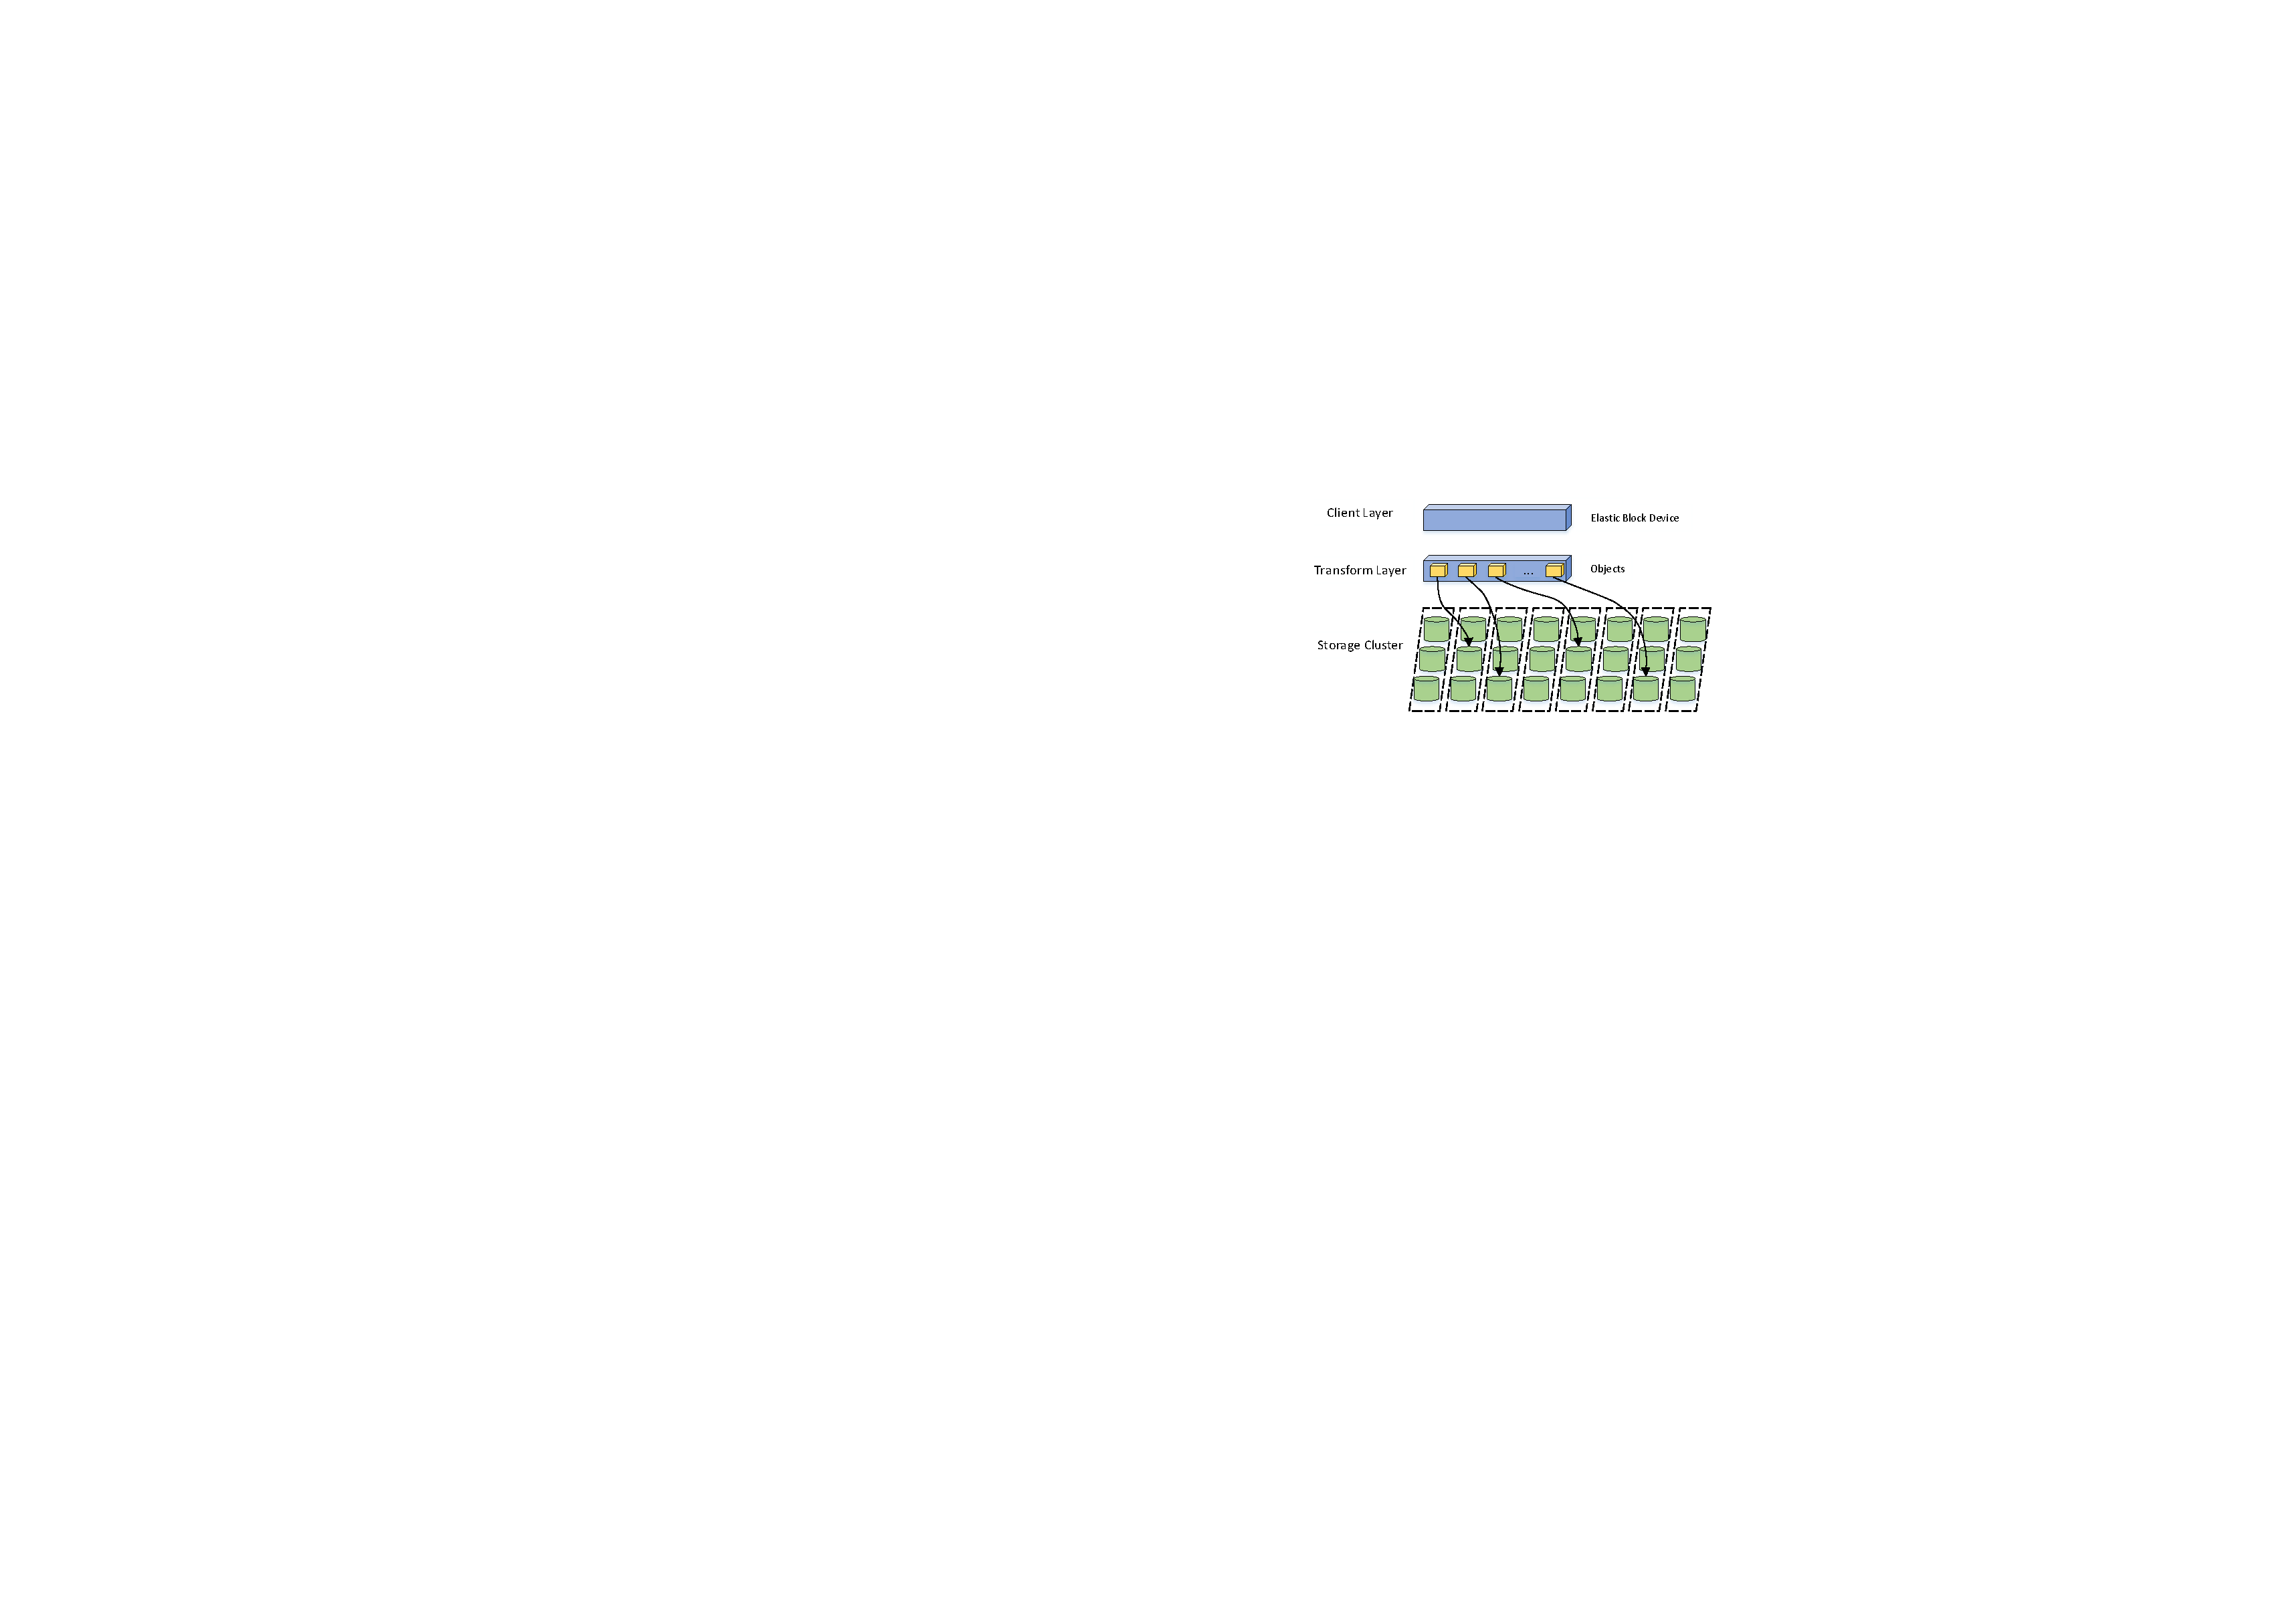
\includegraphics[width=8cm]{figures/ceph_pic/blockdevice.pdf}
	\caption{Architecture of Cloud Block Storage}
	\label{fig:CBS}
\end{figure}
%\vspace{-0.3cm}

\subsection{Snapshot Implementations}
There are many classic snapshot technologies, such as CoW, CoW with
background copy (CoW+), Split Mirror Redundant Array of Independent
Disks (SMRAID), Continuous Data Protection (CDP)
\cite{garimella2006understanding}, and RoW. The different types of
snapshot technologies have been extensively analyzed
\cite{mahipal2021virtual,joseph2019securing,almulla2013distributed,subramanian2014snapshots}. In
summary, the write overhead of CoW, CoW+, and SMRAID are suffered by
their methodologies, their derivative technologies induce overheads
for regular I/O and dramatic increase of sync operations when
snapshots are present \cite{subramanian2014snapshots,li2012irow}. CDP
is mostly dependent on the underlying technology used for taking
snapshots and network bandwidth.


For RoW-based snapshots, new data blocks write to the blocks belonging
to the current snapshot, which stores the root node of the previous
snapshot index for all old data blocks.  RoW sacrifices contiguity in
the original copy for lower overhead updates in the presence of
snapshots.  As the system runs and takes snapshots over a long time,
the fragmentation of the data block becomes increasingly serious. When
locating the data block, the snapshot checks whether it exists in the
snapshot. If not, the snapshot looks for the earlier snapshots by the
root nodes until the data block is located. Thus the process
inevitably increases the number of hops.  Iterative search degrades
performance due to the low update frequency of data blocks and the
massive amount of snapshots.  Snapshot taken by the Google Cloud
Compute Engine Persistent Disk \cite{GoolgeCloudPDS} only contains
blocks that are different from the previous snapshot. Snapshots taken
of the volume in Rackspace Cloud Block Storage
\cite{RackspaceCloudblockstorage} and virtual disk in Microsoft Azure
\cite{MicrosoftAzureVirtualdisk} are incremental snapshots.  Amazon
EBS \cite{varia2014overview} has an optimized RoW snapshot index that
cut off the index dependencies. It copies the entire previous snapshot
index before updating the data blocks. Besides, the index uses a
uniform region to store continuous unmodified data blocks to reduce
the number of nodes.
%	The region points to the last changed snapshot instead of the previous snapshot to avoid iterative queries.
However, this index is not applicable in batch access mode since the
indexes are loaded iteratively.  Moreover, when the number of
snapshots grows, the size of each region shrinks, and the number of
regions grows, the index degenerates into a complete index, which
increases memory overhead.

\subsection{Vary Layers Supported Snapshot}
\begin{table}[htbp]
	\centering
	\caption{Summary of existing methods for the database backup and recovery (FS: file system, DB: database)}
	\label{table:snapshot_layer}
	\resizebox{\columnwidth}{9mm}{
		\begin{tabular}{|c|c|c|c|c|}
			\hline
			Methods       & Mysqldump & Xtrabackup & BTRFS & LVM   \\ \hline
			layer         & DB        & DB         & FS    & Block \\ \hline
			backup speed  & slow      & slow       & fast  & fast  \\ \hline
			restore speed & slow      & medium     & fast  & fast  \\ \hline
	\end{tabular}}
\end{table}

Snapshot technology can be implemented at different layers. Table
\ref{table:snapshot_layer} shows the existing methods supported by
varying layers.  In the database layer, administrator could choose
mysqldump \cite{mysqldump} for logical backup and Percona Xtrabackup
\cite{xtrabackup} for physical backup. A logical backup stores the
queries executed by transactions, while a physical backup copies the
raw data to storage. In the recovery process, the stored queries are
re-executed, or backup data are copied to a database
directory. However, recovery operations in the existing tools take a
long time, since these recovery procedures involve a large amount of
I/O operations induced by database queries. Xtrabackup does not
perform transactions and only copies original data, and then it is
faster than mysqldump in restoring process, but the overhead still
cannot be ignored.

Snapshots techniques supported by file systems and the block layer can
be adopted to the backup and recovery of a database. Network Appliance
NAS filers, the Sun ZFS filesystem \cite{rodeh2003zfs} and BTRFS
\cite{rodeh2013btrfs} organize the file as a tree with data at the
leaf level and meta-data maintained in internal nodes. Each snapshot
consists of a separate tree, but the snapshot may share subtrees with
other snapshots. When the user produces a snapshot of the volume,
simply duplicates the root node of the original volume as the new tree
root node of the snapshot, and the new tree root is pointed to the
same children as the original volume.  Though creating a snapshot is
light, the overhead of first write to a block is heavy because the
entire tree of meta-data nodes needs to be copied and linked to the
root node of the snapshot.  LVM \cite{hasenstein2001logical} operates
between the file system and the storage device and provides fast
snapshot creation and restoration using CoW. However, the CoW approach
negatively affects run-time performance since it performs redundant
writes due to data copies.  We adopt tree structure to organize its
data blocks like Parallax \cite{DBLP:conf/eurosys/MeyerACLFHW08} and
Ramdisk \cite{nielsen1999use} to support rapid creation of snapshots.

\subsection{Characters of Accessing Snapshots}
\label{Characters}
In this subsection, we present our key snapshot observations about the
behaviors of accessing. The characters can be exploited to greatly
help design an optimal snapshot index that accelerates snapshot
restoring and reduces index memory overhead.

As shown in Figure \ref{fig:retained_distribution}, we collect
one-month snapshot information from AliCloud
\cite{alibackupset}. There were 115210 snapshots are preserved in the
first two weeks, 522086 snapshots in the third week, and 634767
snapshots in the fourth week. Most of the snapshots saved in the last
two week, because the system periodically takes snapshots at a fine
density and filters snapshots based on the importance and date, which
means continuously deleting snapshot sets of different lengths rather
than batch deletion.  Besides, earlier snapshots are easily deleted
and merged.  We also count snapshot accessed distribution, as shown in
Figure \ref{fig:accessed_distribution}. There are 2091 snapshots
accessed within the first day, which accounted for 83.4\% of the
snapshots accessed throughout the month. Therefore, the feature of
snapshot accessed is temporal locality.

%At the same time, snapshots are mostly recovered in a continuous manner. 

Auditing and fact-checking \cite{jo2019aggchecker,shaull2008skippy}
are essential for applications now more than ever.  In the multiple
snapshot scenario, the user may retain the most accessed and recent
snapshot set \cite{vrable2009cumulus} to take unanticipated queries on
long-term status.  Besides, snapshots are usually loaded in
deduplication systems as batches
\cite{ren2021accelerating,zou2021dilemma}.  The recovered snapshots
are continuous and the length is indeterminate.  Thus, the access
behavior of snapshots is continuous. This behavior is proper for cloud
tenants, who recover and mount more snapshots on different machines.

%Finally, we observed that the number of snapshots accessed in the last week is 47$\%$ of the snapshots accessed in a month.
%In a short, users typically access the most recent snapshots continuously.

Existing RoW-based snapshot technologies suffer under continuous
access workload. The reason is that the dependency between snapshots
leads to loading all snapshots with reference relationships into
memory instead of only snapshots accessed. The Amazon EBS snapshot
index is a complete tree that stores all region's addresses to
eliminate the dependency. However, it causes significant pressure on
memory consumption because all indexes in memory are complete trees.

%\begin{figure}[t]
%	\centering
%	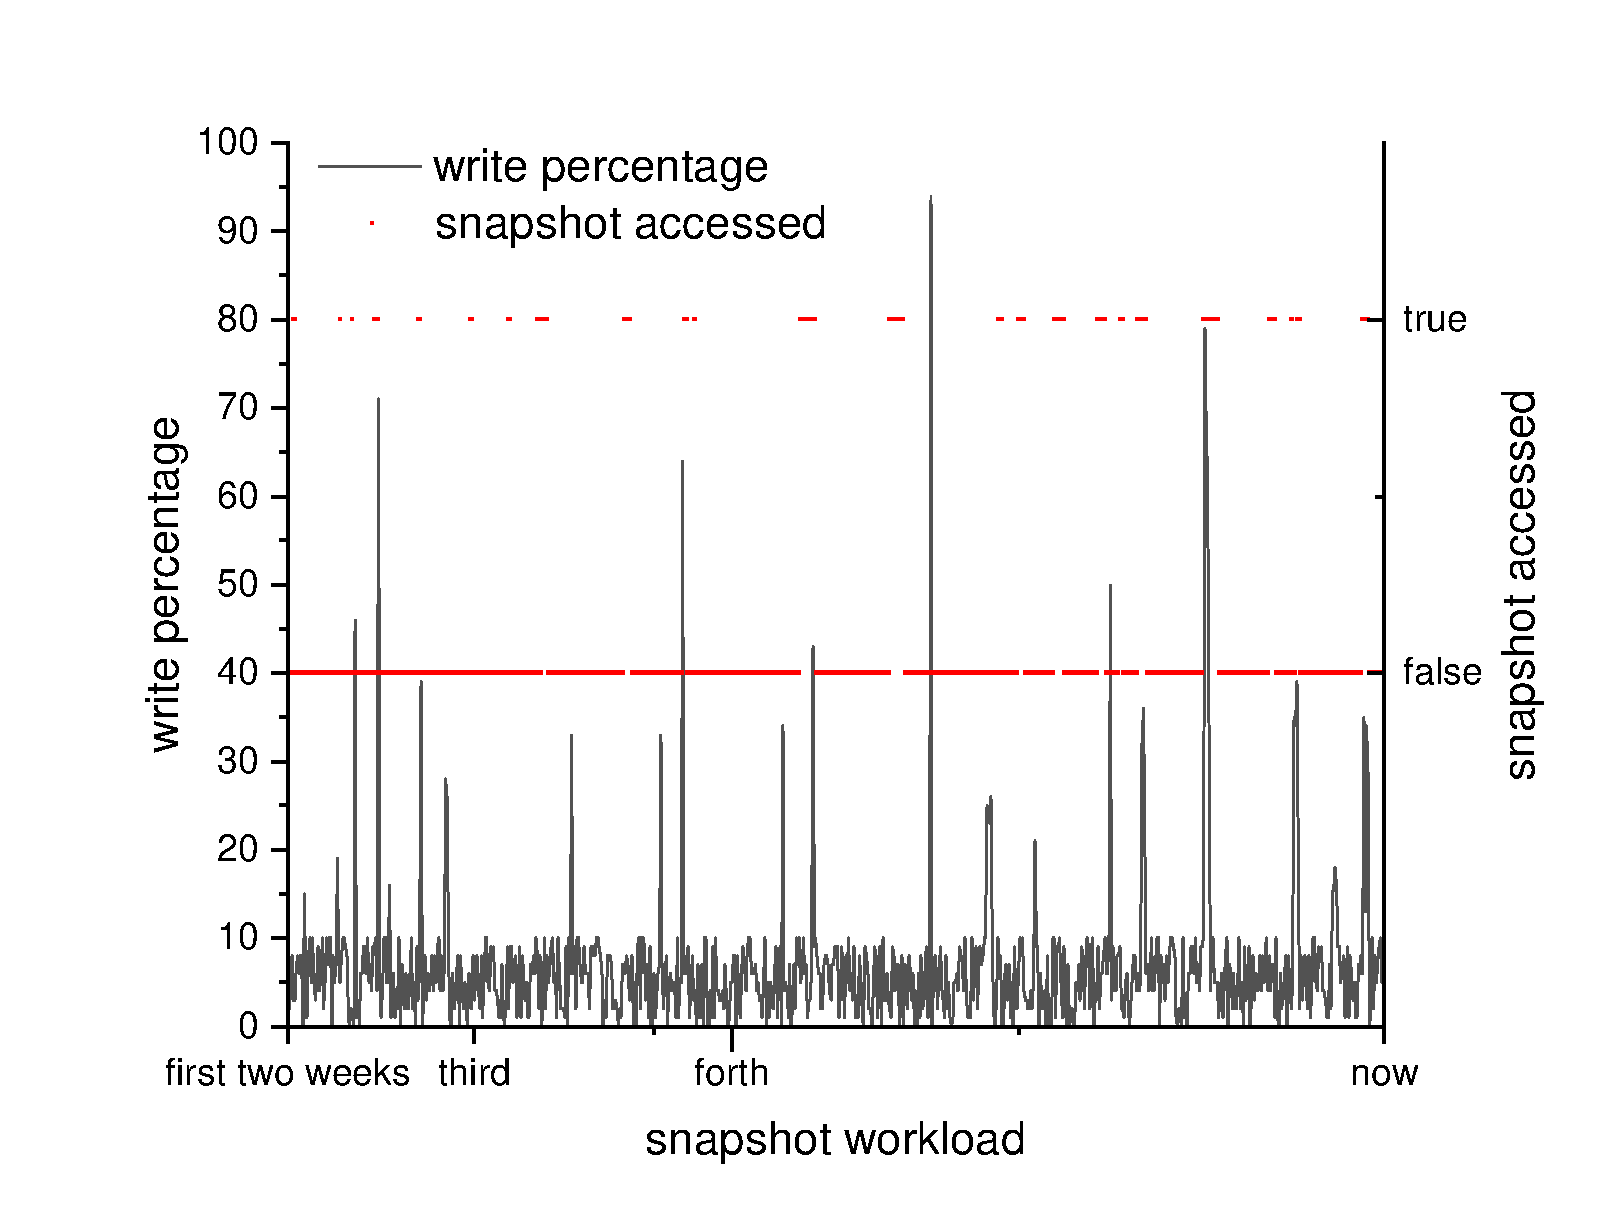
\includegraphics[width=8cm]{figures/ceph_pic/ali_workload.pdf}
%	\caption{Snapshot workload in AliCloud}
%	\label{fig:ali_snapshot_workload}
%\end{figure}
%\vspace{-0.2cm}

\begin{figure}[htbp]
	\begin{minipage}[t]{0.48\linewidth}
		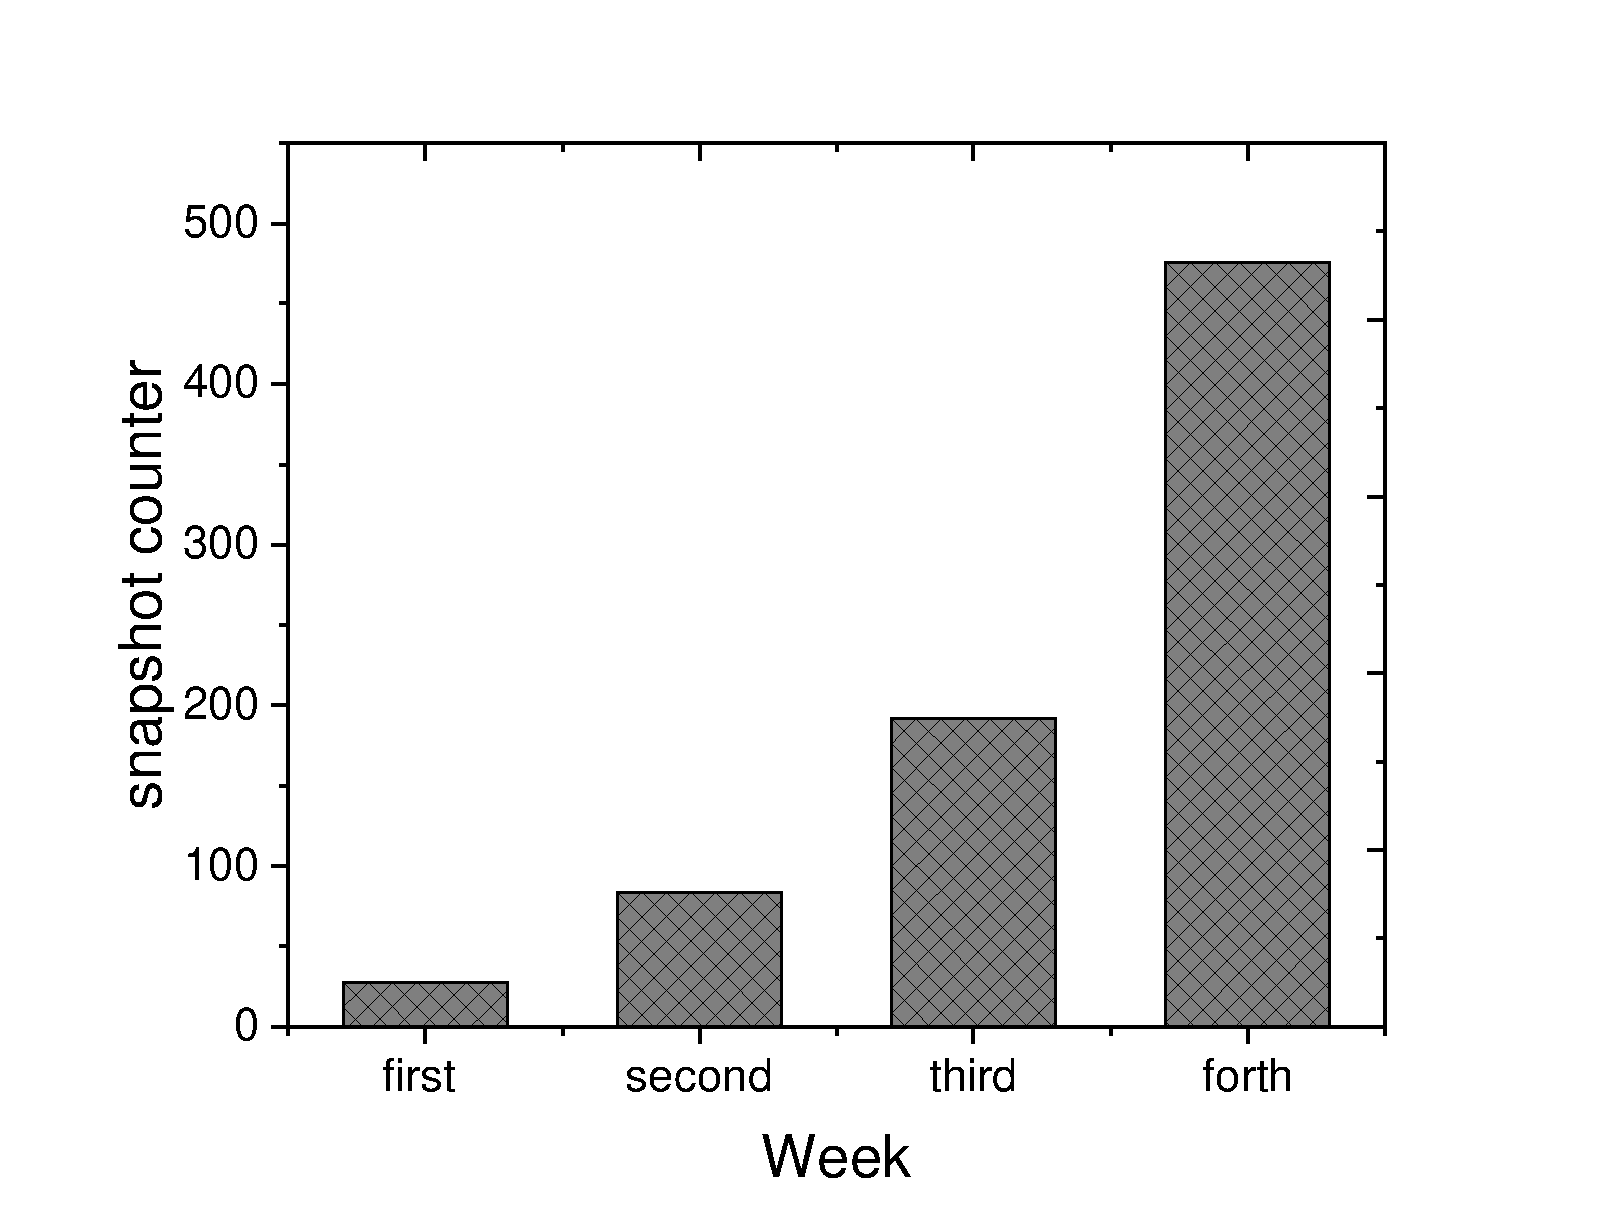
\includegraphics[width=\linewidth]{figures/ceph_pic/ali_counter_workload.pdf} 
		\caption{Snapshot retained distribution} 
		\vspace{-0.3cm}
		\label{fig:retained_distribution}
	\end{minipage}
	\hfill%
	\begin{minipage}[t]{0.48\linewidth}
		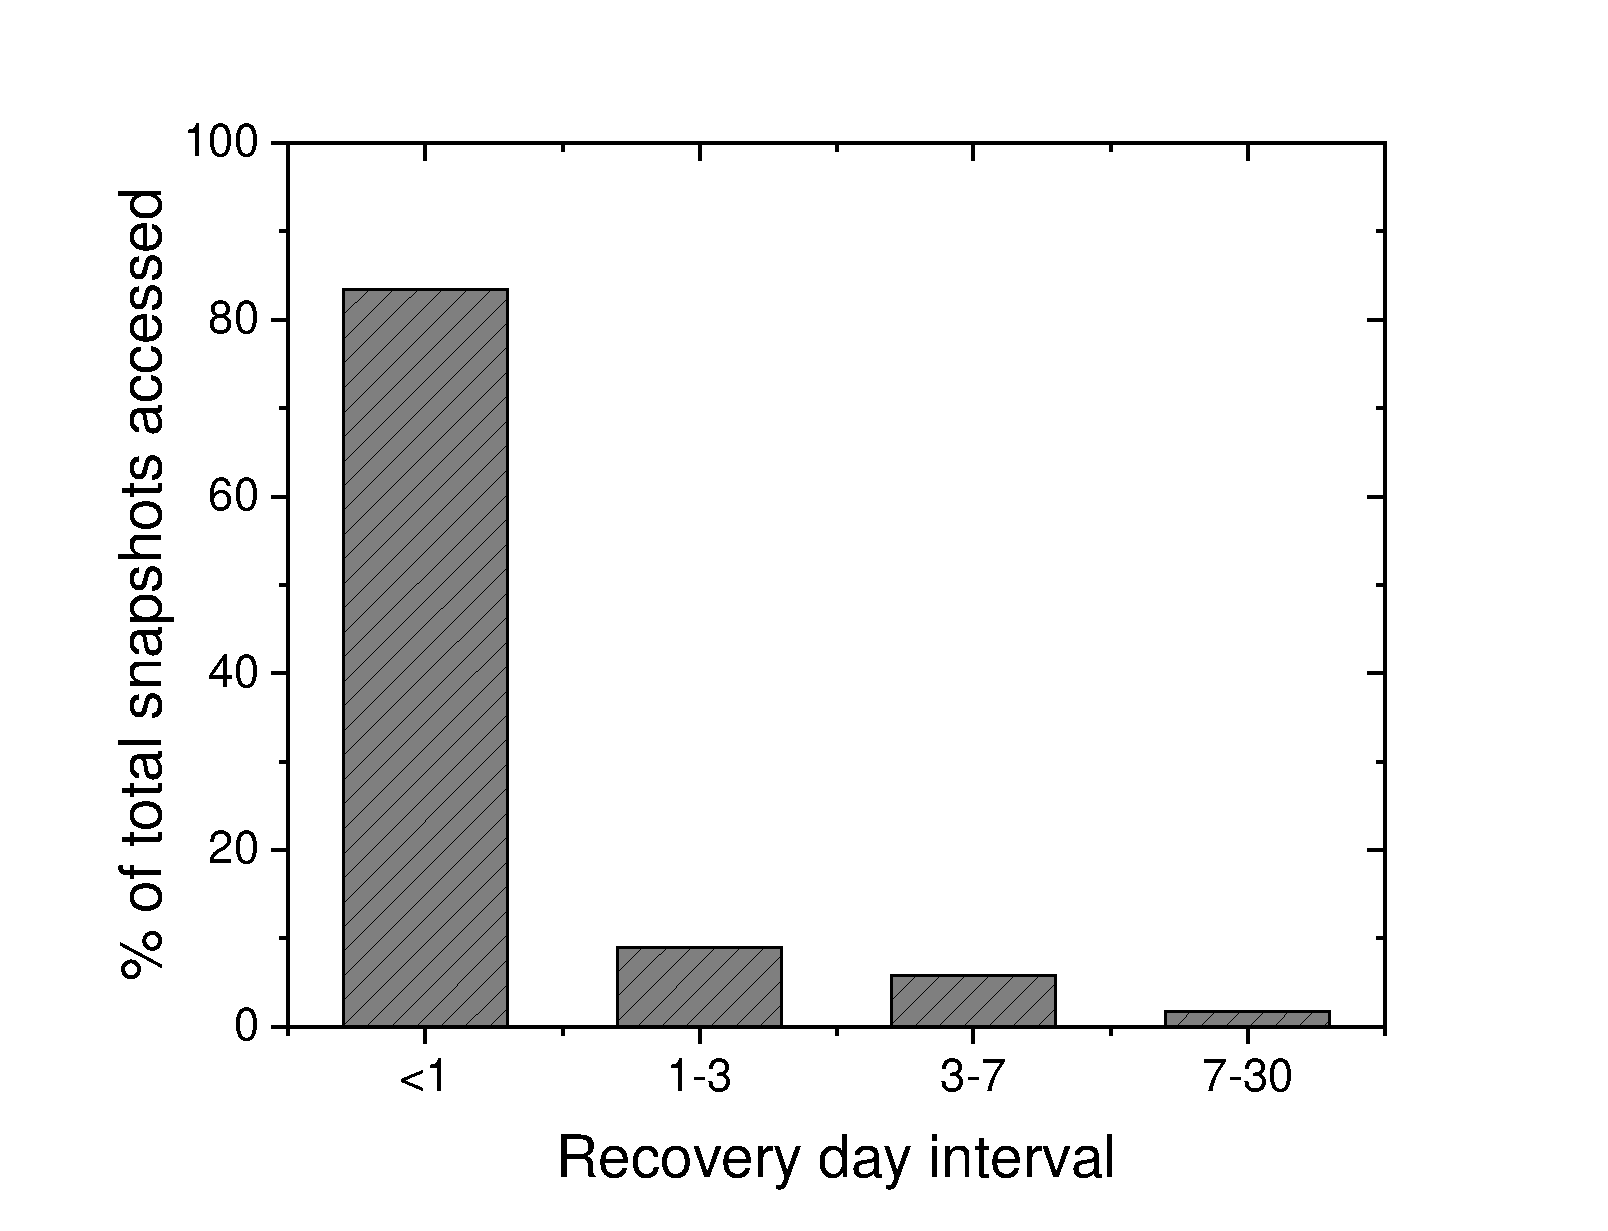
\includegraphics[width=\linewidth]{figures/ceph_pic/ali_percentage_workload.pdf}
		\caption{Snapshot accessed distribution}
			\vspace{-0.3cm}
		\label{fig:accessed_distribution}
	\end{minipage} 
\end{figure}
\vspace{-0.3cm}



\section{Motivation}
\label{Motivation}

\subsection{Fragmentation and Iterative Traversal}
As discussed in Section 2, fragmentation causes serious iterative
traversal in snapshot versions based on the RoW technique. In this
subsection, we analyze the reason of iterative traversal with a typical
example.

\begin{figure}[htp]
	\centering
	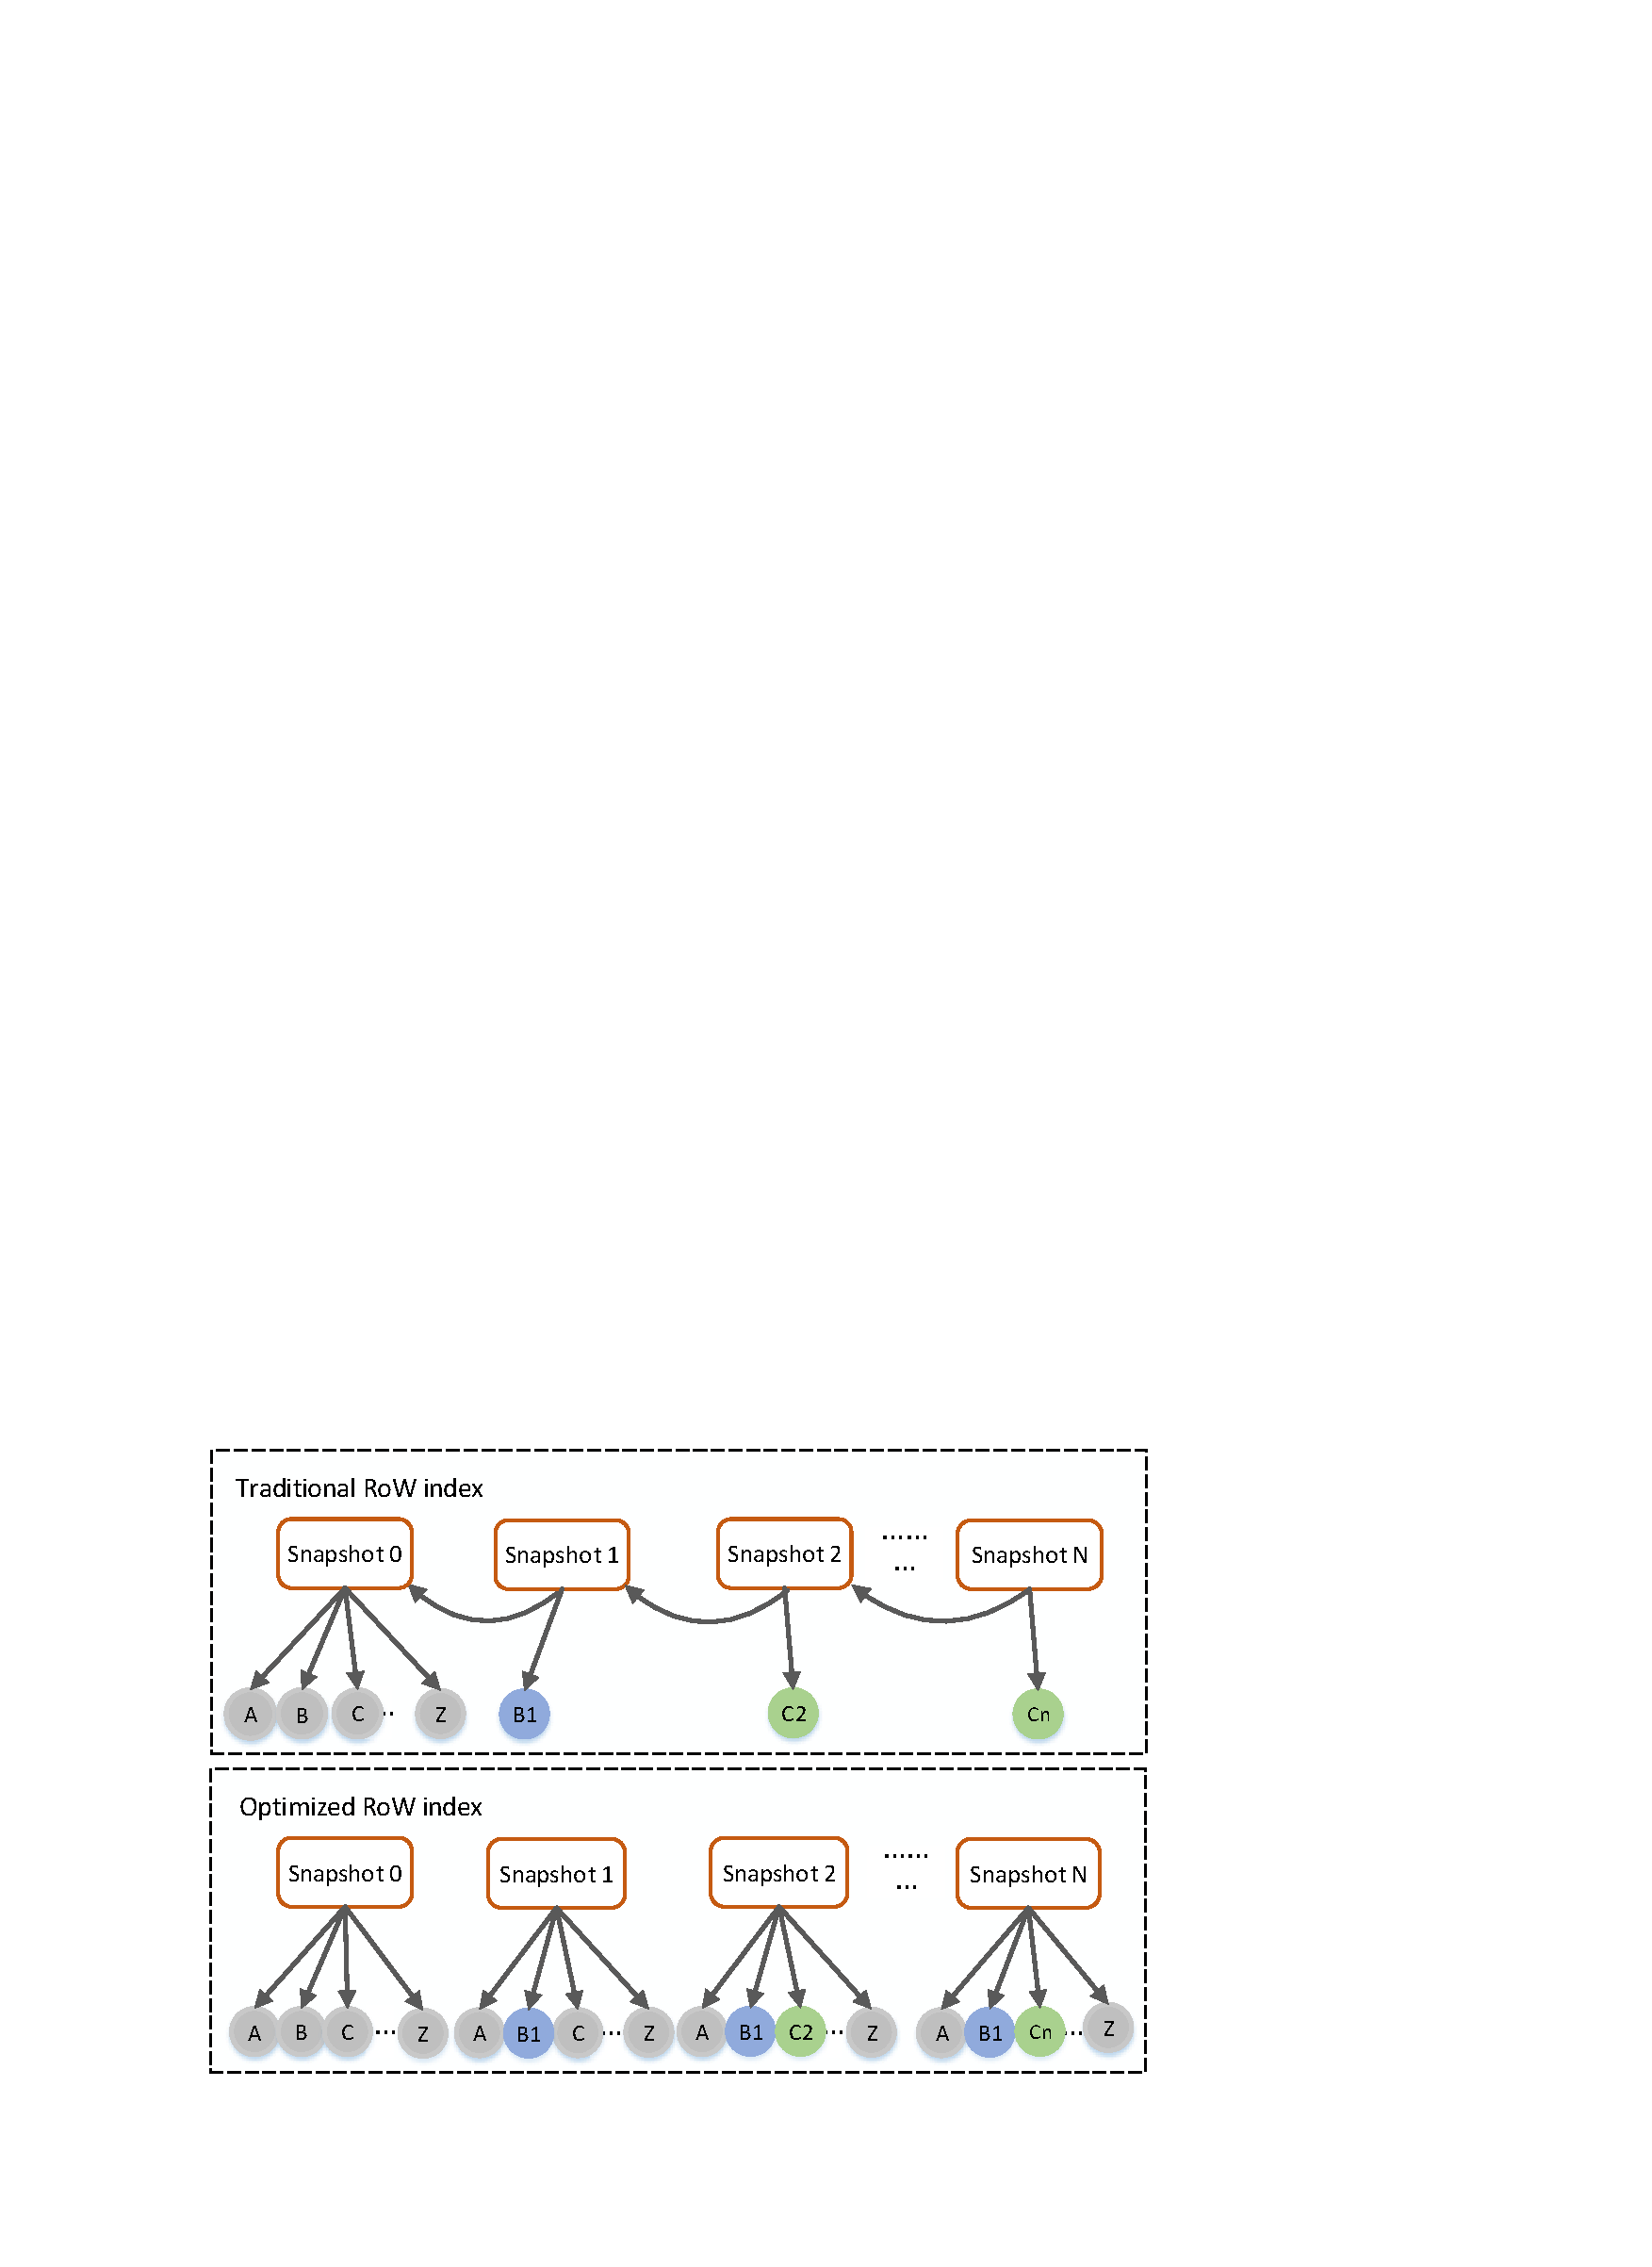
\includegraphics[width=\columnwidth]{figures/ceph_pic/orig_RoW_and_OpRoW.pdf}
	\caption{Example of unbounded traverses to restore snapshots on traditional versus optimized RoW index}
		\vspace{-0.3cm}
	\label{fig:row-index-vs}
\end{figure}



In traditional RoW, the root node points to the root node of the
previous snapshot index, and new data blocks are written to the
current snapshot. During the snapshot recovery phase, the recovery
process requires access to other snapshots because the data blocks of
the snapshot are scattered in other snapshots rather than only the
current snapshot. The first step in locating an unmodified data block
is to verify the destination snapshot, and then check the existence of
the data block. As shown in Figure \ref{fig:row-index-vs}, there are
\emph{Block A}, \emph{B} until to \emph{Z}. \emph{Block B} is updated
in \emph{snapshot 1}, \emph{Block C} is updated in \emph{snapshot
2}. When restoring \emph{snapshot 1}, only \emph{snapshot 0} and
\emph{snapshot 1} are verified. However, when restoring \emph{snapshot
N}, the recovery process first checks \emph{Block A} in \emph{snapshot
N-1} while \emph{Block A} is not updated in \emph{snapshot N-1}. The
recovery process has to access previous snapshots iteratively until
found in \emph{snapshot 1}. For \emph{Block B}, the same traversal
path is required. The recovery latency is affected by the data block
fragmentation and the number of snapshots.  For the optimized RoW, in
Figure \ref{fig:row-index-vs}, the snapshot copies all snapshot
numbers for unmodified data blocks at the end of the snapshot period.
However, each snapshot index is a complete tree, which puts
significant pressure on the memory overhead of the client node and
snapshot loading from the storage cluster due to the snapshot access
characteristics.

Amazon EBS \cite{varia2014overview} relieves memory pressure by
replacing leaf nodes with regions based on the optimized RoW index.
However, when the fragmentation of the data block increases, the size
of the region is dropping while the number is increasing. Thus the
index degenerates into the complete index which significantly boosts
the memory usage. Under the snapshot feature of continuous accessing,
EBS needs to iteratively load multiple snapshot indexes in distributed
storage.

\subsection{Optimal Snapshot Index}
Under the observations and comparisons of existing snapshot indexes,
fragmentation caused serious iterative traversal in snapshot versions
based on the RoW technique.  We present an optimal snapshot index
namely GSnap, which cuts off the reference by putting the snapshot
indexes into the group to eliminate iterative traversal.

\textbf{An example of GSnap:} For the \emph{snapshot 1}, \emph{2},
\emph{3}, we put them into a group. \emph{Snapshot 1} records the
modified data block during the snapshot period, namely \emph{Block
B1}, and records all unmodified data blocks since it is the first
snapshot in this group, thus its index is a complete tree.  The
\emph{snapshot 2}, \emph{3} no longer need to store addresses of the
unmodified data blocks any more, and only store \emph{Block C2} and
\emph{C3} respectively. When restoring a snapshot, we load the group
into memory that means all snapshots in the group are restored. The
snapshots after this group are divided into individual groups, which
are organized similarly. The rationale behind this is to cut off the
reference relationship between two groups while implementing
incremental snapshots in a group. Only snapshots within the group need
to be accessed to avoid iterative traversal when looking up the
address of a data block.

\begin{figure}[htp]
	\centering
	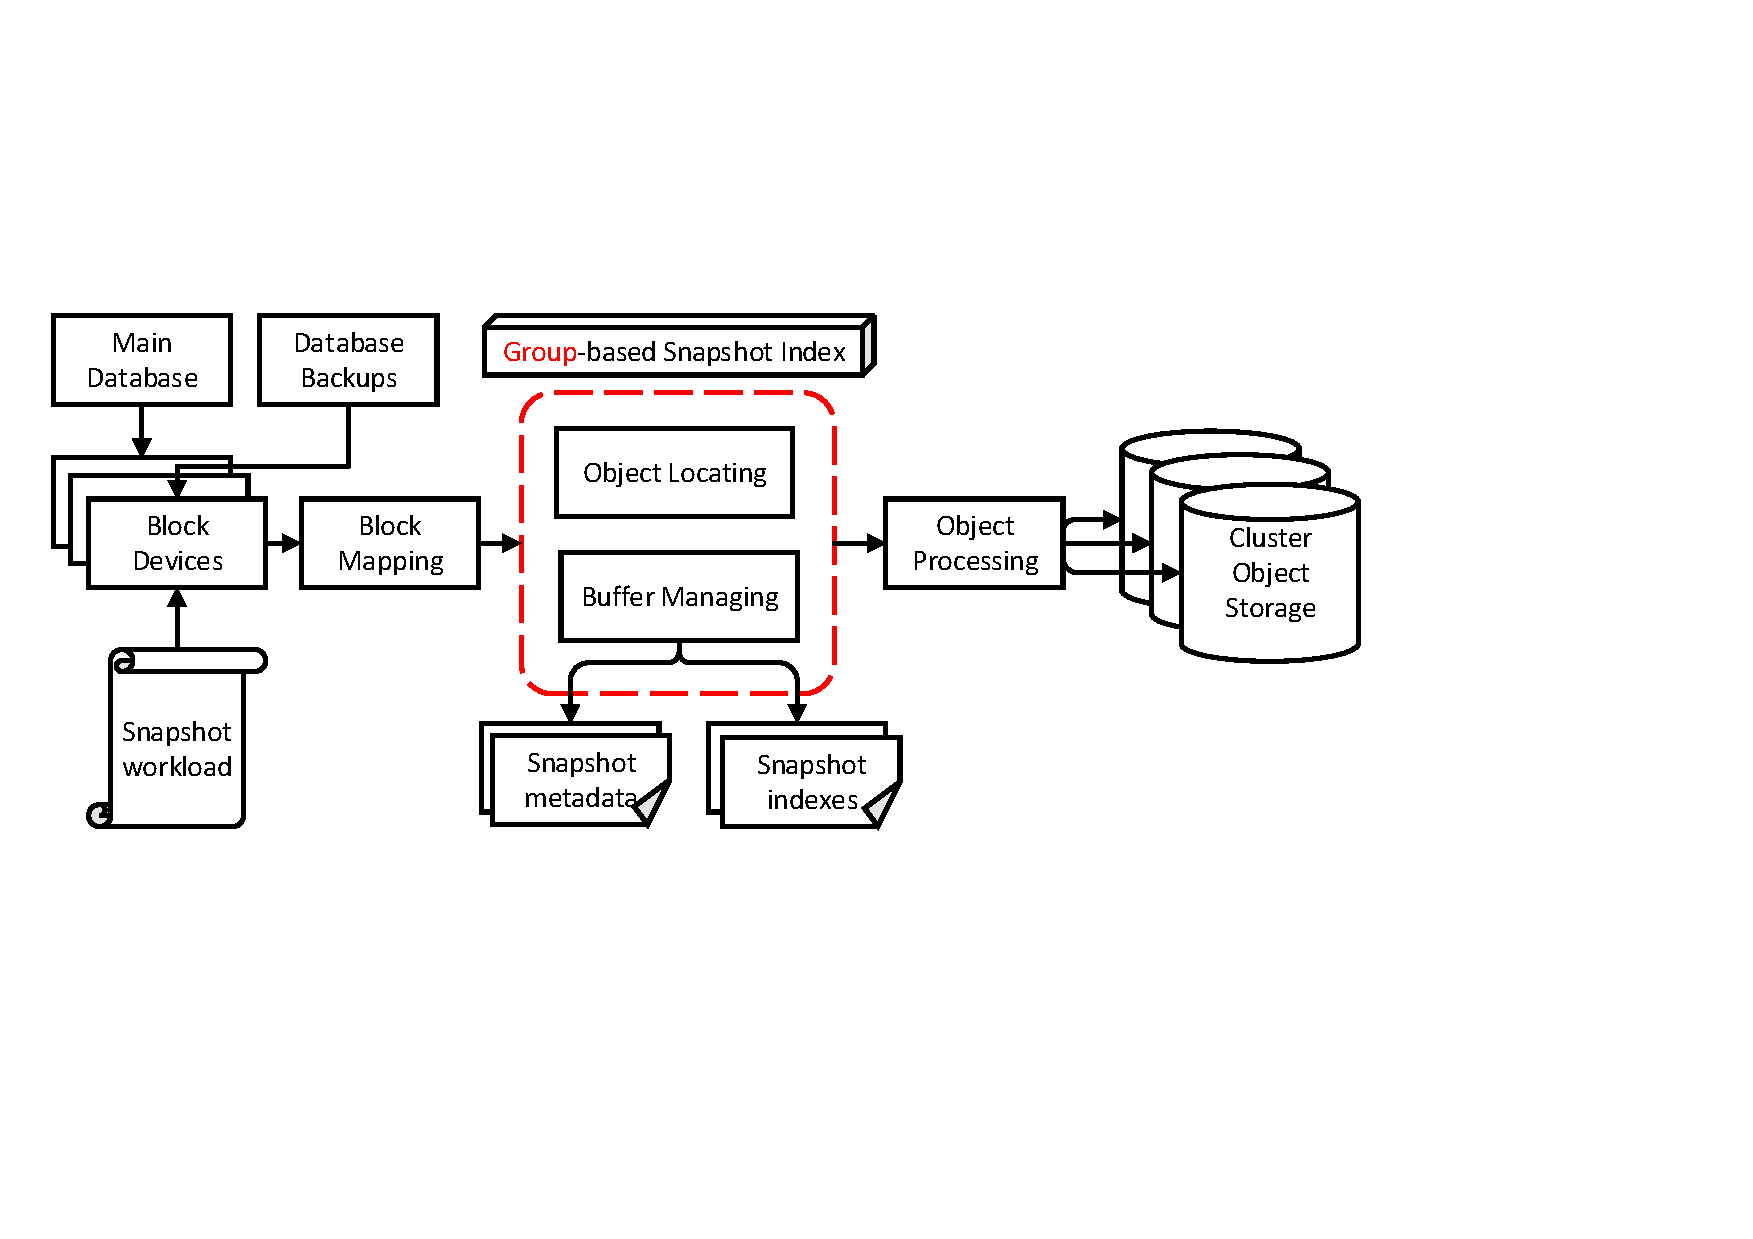
\includegraphics[width=\columnwidth]{figures/ceph_pic/arch_overview.pdf}
	\caption{An overview of GSnap index framework}
	\label{fig:framework}
\end{figure}

\textbf{GSnap framework overview:} GSnap manages the indexes within
the group by using two key techniques. The overall workflow of the
GSnap framework is shown in Figure \ref{fig:framework}, which includes
three key stages: \emph{Block Mapping}, \emph{Indexing}, and
\emph{Object Processing}.
\begin{figure*}[htp]
	\centering
	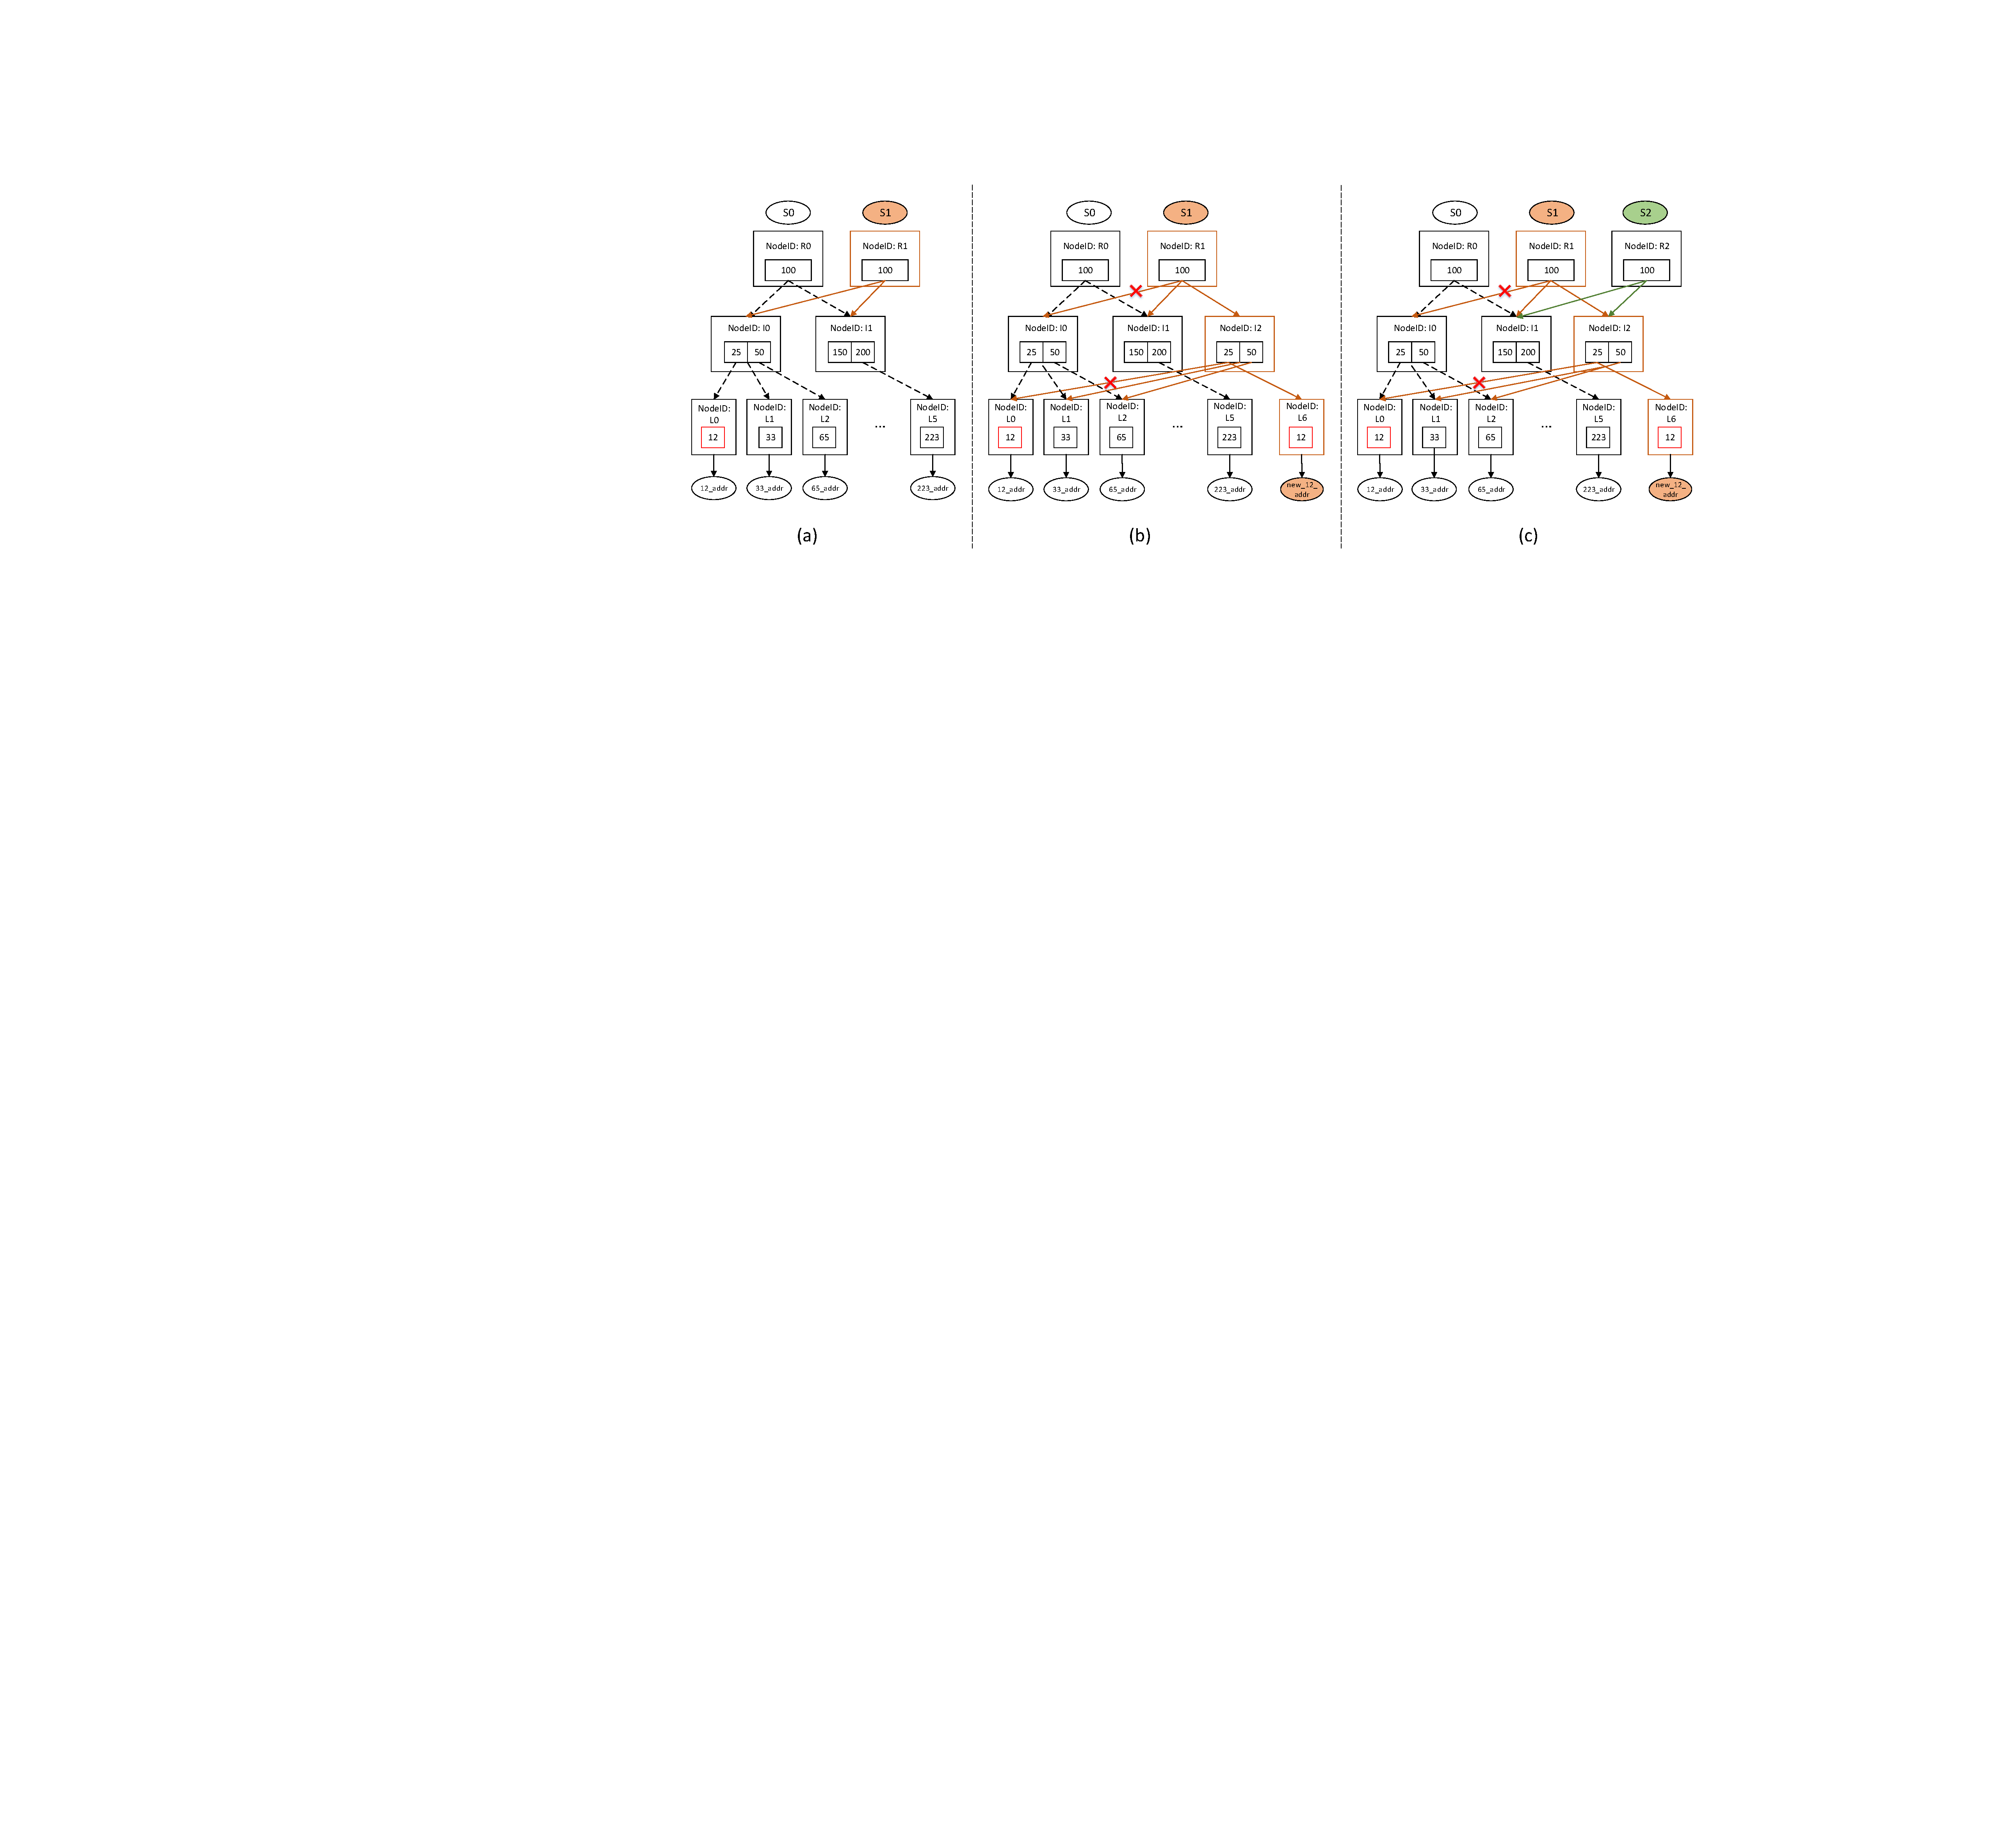
\includegraphics[width=16cm]{figures/ceph_pic/snaptree.pdf}
	\vspace{-0.2cm}
	\caption{SnapTree: \textbf{(a)} Create S1 snapshot. \textbf{(b)} Block No.12 data write. \textbf{(c)} Create S2 snapshot}
	\label{fig:snaptree}
\end{figure*}


\begin{itemize}
	\item \textbf{Shared-Subtree Indexing(SSI)}. The snapshot
          index is organized in the B+ tree structure and the leaf
          nodes store the addresses of the data blocks. SSI shares the
          internal and leaf nodes among the indexes. Hence, we only
          need to build and insert nodes when data blocks are modified
          to maintain that the path from the root node to the leaf
          node is complete, as detailed in Section \ref{SSI}.
	\item \textbf{Group-Based Dividing(GBD)}.  GSnap triggers GBD
          once the data blocks updated in the group are saturated. GBD
          initializes the state of the new group to the active and
          flushes the achieved group to the storage
          cluster. Specifically, GSnap allocates the data block budget
          and sets the length of the group by Algorithm
          \ref{algorithm:dividing}, as detailed in Section \ref{GBD}.
\end{itemize}
Block Mapping refers to the read/write requests of the database being
mapped to the logical blocks of the block device through the Linux
Storage Stack(LSS). The block device can be Rados Block Device(RBD)
\cite{weil2006ceph} or Network Block Device(NBD). Indexing accelerates
the mapping of logical block numbers to physical blocks. Object
Processing indicates that the subsequent requests are processed
asynchronously via transactions after the network connection is
established with the target object storage node. Write operation
requests are duplicated across multiple nodes.  In general,
group-based snapshot index consists of two parts, data block locating
and cache management. Data block locating works in snapshot accessing
and group restoring.  The cache loads snapshot indexes based on the
access characteristics and adopts the LRU algorithm to swap out the
snapshot group, which effectively reduces the index memory overhead.

\textbf{Challenges for GSnap.} Actual snapshot workloads are much more
complicated than the example shown in Figure \ref{fig:row-index-vs},
this results in inconsistent update frequency in each snapshot. Then
the number of updated data blocks and the length of group are the key
factors for taking and restoring snapshots.  The update delay and
memory usage of the index are proportional to the number of data
blocks, we set the block budget for the latter group based on the
block consumption of the former group to reduce memory overhead.  The
snapshot group length is still rewarded by the the former group so
that ensure the indexes of each group occupy a close memory size for
stable snapshot recovery and simple memory management. Besides, as we
know from the previous section that users access snapshots
continuously, we tend to set the length of the group is equal to the
recent average access length of snapshots. We analyze those factors in
detail in the next section.

\vspace{-0.3cm}
\section{Design and Implementation}
\label{Design}
%	In this section, we dissect how SSI and GBD work to cut off
%	the reference and determine the size of the group. In
%	addition, we also theoretically analyzed the size of the group
%	and cache management, and finally analyzed the snapshot
%	deleting and group index merging.

\subsection{Shared-Subtree Indexing}
\label{SSI}
Snapshots also organize data blocks like the file system through a
tree. The addresses of data blocks are stored in the leaf nodes. The
root node and internal nodes point to the next level nodes, and the
key in the node is the ID of the data block. Moreover, we set an ID
namely \emph{NodeID} for each node in the tree.  The index just copies
the root node of the last index as the new root node, which may share
subtrees with other indexes once the user creates a snapshot.  Data
blocks shared with the snapshots can not be updated in place when
write operations to a block device come.  All writes must be
redirected to new data blocks created by the current snapshot. The
index creates leaf nodes for new data blocks, then checks whether the
path from the leaf nodes to the root node is complete. If not, the
index duplicates the internal nodes from the previous index, and
finally modifies their pointers to redirect to the new leaf
nodes. However, the nodes that record unmodified block numbers still
point to the prior indexes.


We show SSI with an example in Figure \ref{fig:snaptree} (a), when the
user takes the snapshot \emph{S1}, it just copies the root node from
the snapshot tree \emph{S0}, as the new root node namely \emph{R1},
and \emph{R1} points to the internal nodes \emph{I0} and \emph{I1}
instead of pointing the root node \emph{R0}.  Figure
\ref{fig:snaptree} (b) shows that block \emph{No.12}, whose address is
recorded by the leaf node \emph{L0}, is updated in the snapshot
period. Specifically, \emph{S1} creates a new leaf node \emph{L6} and
stores the address of the new block, then checks whether the path from
the root node \emph{R1} to the target leaf node \emph{L6} is
complete. If not, \emph{S1} copies all internal nodes from \emph{R1}
to \emph{L0}, and then changes the pointers to redirect to those new
nodes. The root node \emph{R1} points to internal node \emph{I0} and
changes to point to new internal node \emph{I2}, then \emph{I2}
redirects to leaf node \emph{L6} instead of \emph{L0}. In the same
way, the root node \emph{R2} points to internal nodes \emph{I1} and
\emph{I2} when taking the \emph{S2} snapshot.

There are two advantages of the shared subtree structure.  First, the
subtree sharing among snapshots makes locating leaf nodes on any
snaptree in the group with a constant time. The reason is that the
number of hops to locate a leaf node is the same as the height of the
tree regardless of the number of snapshots.  Second, the memory
footprint occupied by the tree is proportional to the number of
updated data blocks in this snapshot instead of storing all nodes in
each tree, and the index redundancy is reduced by only saving one copy
of the address.
% the physical address of the data block in any snapshot can be directly accessed.

\subsection{Group-Based Dividing}
\label{GBD}
In this subsection, we introduce the Group-Based Dividing method,
which is designed to cut off the snapshot index dependency and
establish snapshot recovery granularity.  There are two stages in GBD,
the snapshotting stage and the dividing stage.  In the snapshotting
stage, the snapshot indexes generated in the group are partial
trees. Besides, the state of the last index is \emph{active} while
others are \emph{achieved}.  In the dividing stage, the first snapshot
index generated in the next group is a complete tree. The state
transformation between the two stages is determined by the update
ratio of the snapshots in the group and the latest average continuous
access interval.

\textbf{Snapshotting stage.} In this stage, the system only copies the
root node of the previous snapshot index for the new snapshot
index. The new root node points to all internal nodes of the previous
index and the number of snapshots in the group $S$ plus 1.  Besides,
the \emph{Created} flag of all internal nodes in the index are reset
to false, which implies that no nodes are created in the index yet.
As shown in Figure \ref{fig:snapshotgroup_devide}, when the data
blocks updated dose not reach the saturation, the snapshot index $S_1$
only copies one root node, the reference of all leaf nodes in previous
index is incremented by 1.  At the same time the previous index status
is converted to \emph{achieved}, and the current snapshot index status
is \emph{active}, which means all writes are updated in the current
snapshot and only the current index could be modified during the
period.  We collect the update ratio of the former group $P$ after the
group state is changed.  Once a data block is updated, the block
counter $O$ recorded in group increase by 1 and the \emph{Created}
flag of the new added internal nodes is set to true.


\textbf{Dividing stage.} When the number of snapshots $L$ or the block
counter $O$ in the group reaches the threshold, the group state
transforms into the dividing state. $L$ and $O$ are factors to trade
off the recovery speed and memory overhead, and they will be discussed
in Section \ref{section:Recovery model}. Figure
\ref{fig:snapshotgroup_devide} shows that the snapshot index $S_n$
traverses all the leaf nodes of $S_{n-1}$ and constructs a complete
tree.  Since traversing the leaf nodes only needs to access the root
node of the last snapshot index and the number of hops is fixed, which
speeds up the construction of the tree.  The internal nodes updated in
the last tree are marked. The system additionally copies the latest
child nodes to the next group to reduce the delay in building a
complete tree.  GSnap allocates the block budget and set group length
to the latter group based on the block consumption of the former group
and the latest average continuous access snapshot length namely $C$.
We constrain the continuously accessed snapshots in a group and adjust
the size of the group based on the update ratio of snapshots.  As
shown in Algorithm \ref{algorithm:dividing}, GSnap compares the block
budget $O^\ast$ with the block counter $O$ and set the block and group
length budget of the latter group. If the block counter $O$ equals the
block budget $O^\ast$, that means the block budget has been exhausted
and the length of the group has not reached the threshold. GSnap
rewards the latter group with the same update ratio and does not
change the group length budget. The latter group is punished if the
block budget is not used up, and the length budget is decreased to
$p$, and $p$ is the punish factor. In addition, we take the maximum
value between $L_{n+1}$ and the average continuous access length $C$
to cover the snapshot set.




\begin{algorithm}[htp]
	\caption{GSnap Index Group Dividing}
	\label{algorithm:dividing}
	\KwIn{$C$ - The latest average continuous access snapshot
		length;
		$O_n^\ast$ - The object budget in the $n$-th group;
		$L_n^\ast$ - The snapshot budget for the $n$-th group;
	}
	\KwOut{$SC_n^\ast$ - A set which stores pairs from snapshot to
		modified block count in the $n$-th group;
		$O_{n}$ - The number of modified objects in the $n$-th group;
		$L_{n}$ - The number of snapshots in the $n$-th group;
		$P_{n}$ - The average update ratio of the $n$-th group;
		$O_{n+1}^\ast$ - The object budget in the $(n+1)$-th group;
		$L_{n+1}^\ast$ - The snapshot budget for the $(n+1)$-th group;}
	
	init $SC_n$, $O_n$, $L_n$, $P_n$;\\
	\While{$O_n^\ast$> $O_n$  $\&\&$ $S^\ast$.siz >= $S_n$}{
		do taking snapshot and updating index;\\
		$SC_n$.insert(snapid, count);\\
		update $O_n$, $L_n$, $P_n$;\\
	}
	\eIf{$O_n$ $\geq$ $O_n^\ast$}  
	{
		$L_{n+1}^\ast=\max(L_{n}, $C$)$;         // length reward \\ 
	}
	{
		$L_{n+1}^\ast=\max(p\times L_{n}, $C$)$;         // length punish\\
		
	}
	\hspace*{0.2in} split the group, and transform achieved group; \\
	\hspace*{0.2in} $O_{n+1}^\ast=L_{n+1}^\ast \times P_n$;\\
	return $L_{n+1}^\ast$, $O_{n+1}^\ast$;\
\end{algorithm}



\begin{figure}[htp]
	\centering
	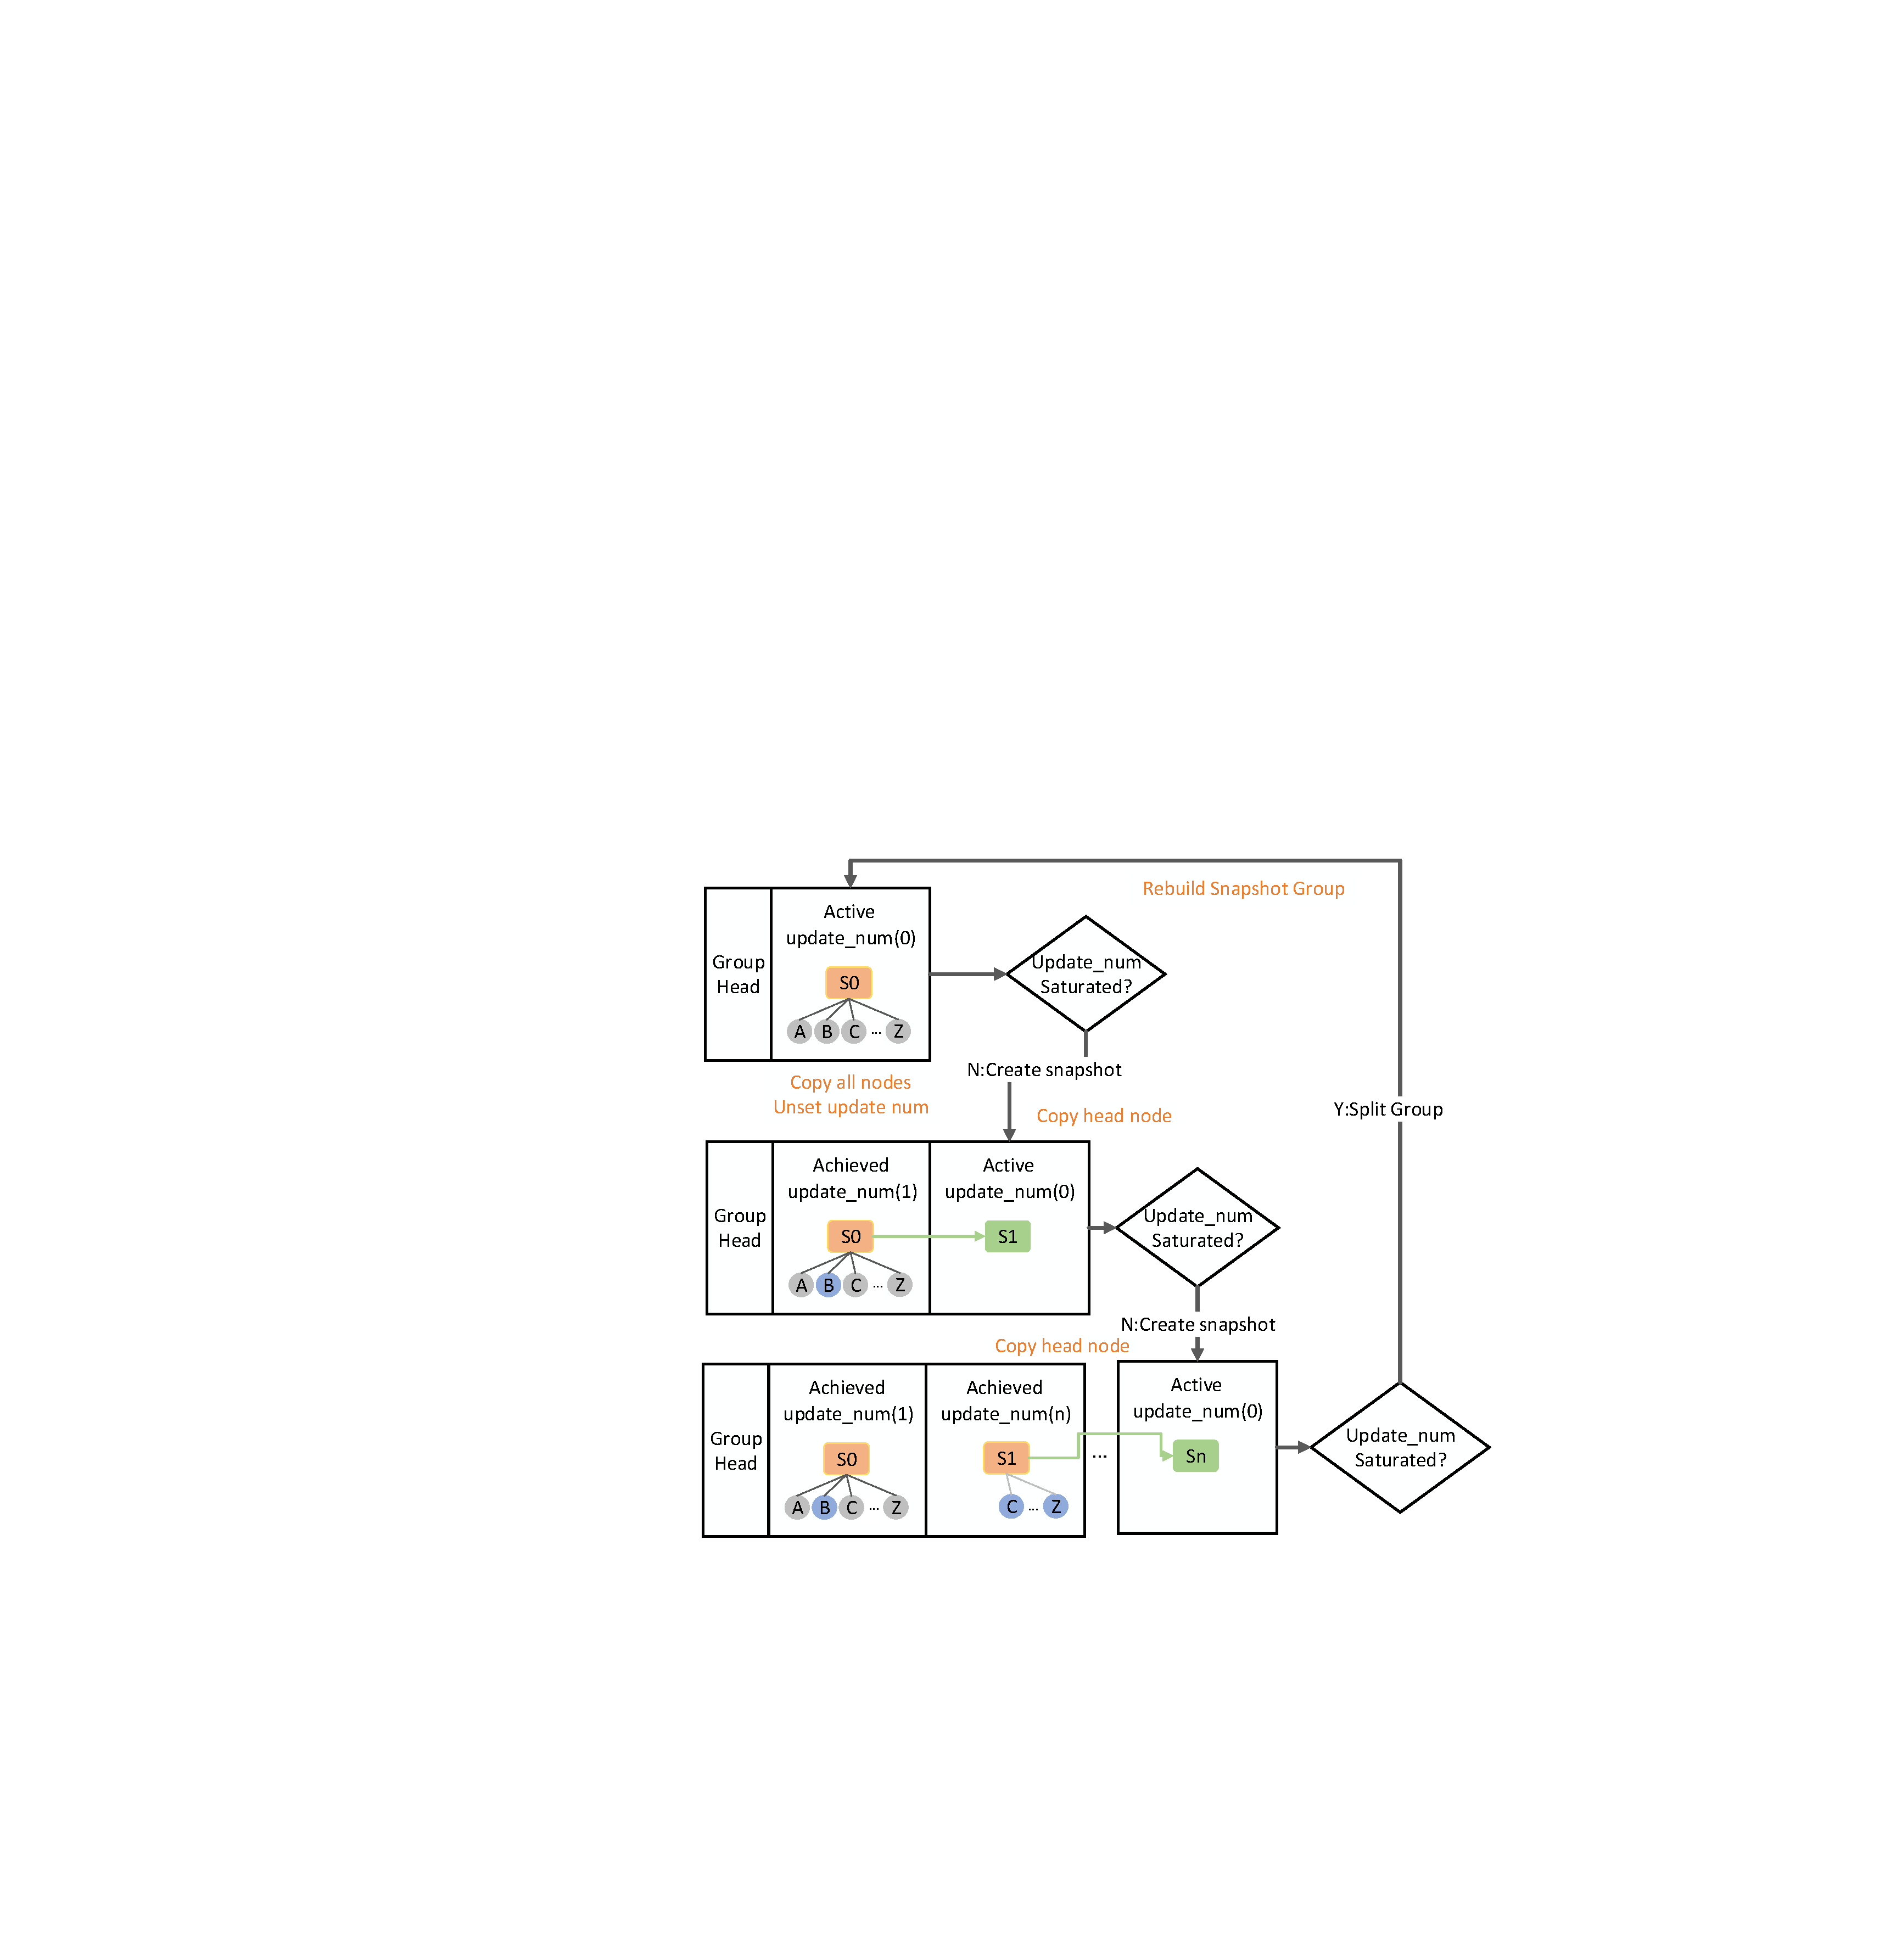
\includegraphics[width=\columnwidth]{figures/ceph_pic/group_divide.pdf}
	\caption{An example of GSnap index division}
	\vspace{-0.3cm}
	\label{fig:snapshotgroup_devide}
\end{figure}


\subsection{Cache Management of GSnap}
In this subsection, we introduce how to access the data blocks and
cache management of the client host.

GSnap uses the shared memory to cache the snapshot index, which is
appropriate for the interprocess communication. And the user could
adjust the shared memory size to accommodate the snapshot size and
access frequency by the profile.  When mounting a block device, a
daemon process is started in the system for data block locating and
index cache management.  As shown in Figure \ref{fig:cache_managment},
the daemon process allocates and initializes the memory space, which
include four partitions: \textcircled{1} \emph{SM\_Admin} includes
$Cache\_Allocter$ and shared memory metadata, such as total space
size, number of groups, etc. $Cache\_Allocter$ is responsible for the
expansion of shared memory. The metadata is used to allocate memory
segments to the group index and adopt LRU replacement algorithm to
swap out the least recently accessed group index; \textcircled{2}
\emph{Snap\_Admin} stores group metadata, and it is responsible for
locating and loading the snapshot groups; \textcircled{3} the snapshot
index in the latest group from the storage node is loaded in
\emph{Latest\_Group}, which refers to the snapshot index that has not
yet formed a group; \textcircled{4} the left space is used as a heap
to store the indexes of groups.

When accessing the snapshot set, the daemon process checks whether the
set has been loaded into memory. As shown in Algorithm
\ref{algorithm:locate}, \emph{Snap\_Admin} compares the snapshot set
$NL$ with the group set $AL$ that already loaded into memory.  If
$coverd$ is true and $NS$ is empty, target snapshot set indexes have
been loaded into memory. $NS$ contains all the snapshot segments which
are needed to be loaded.  Otherwise the daemon process traverses $NS$
and $Group\_Set$ to determine the groups need to be loaded. Finally,
\emph{Snap\_Admin} finds the addresses of the index groups in
$Group\_Addr\_Set$, and actively loads them from the cluster into the
shared memory.  We use $Group\_Access\_Counter$ to count the number of
accesses of the snapshot groups. Once the shared memory is not enough,
we adopt a simple LRU algorithm to swap out the least recently
accessed index group, and the granularity of swap out is the group
instead of the snapshot.

\begin{algorithm}[htbp]
	\caption{Index Group Checking}
	\label{algorithm:locate}
	\KwIn{$AL$ - A sorted set includes all pairs from group start
          to end snapshot id, and groups have been loaded into memory;
          $NL$ - The pair of snapshots to be accessed, including the
          start to end snapshot id;
		
	} \KwOut{$covered$ - Whether to cover; $NS$ - A linked list
          includes all snapshot segments need to load, including the
          start to end snapshot id; }
	
	init $covered$, $NS$, rear=$GS$.size;\\
	\eIf{$AL(0).first \leq NL.first $ \&\& $ NL.second\leq AL(rear).second$}
	{
		\ForEach{AS in NL}{
			\If{$AS.first \leq NL.first$ \&\& $AS.second \geq NL.second$ }{
				$coverd$ = true;\\
				break;\\
			}	
			\eIf{$AL.first \geq NL.first$ \&\& $AS.second \leq NL.second$}{
				$NS$.append($NL.first$, $AS.first$);\\
				$NS$.append($AS.second$,$ NL.second$);\\
			}{
				
				$NS$.append(max($NL.second$, $AS.first$), max($NL.first$, $AS.second$));
			}
			
		}
		
	}
	{
		$NS$.append(uncovered set);\\
	}
	return $coverd$, $NS$;
\end{algorithm}

\begin{figure}[htbp]
	\centering
	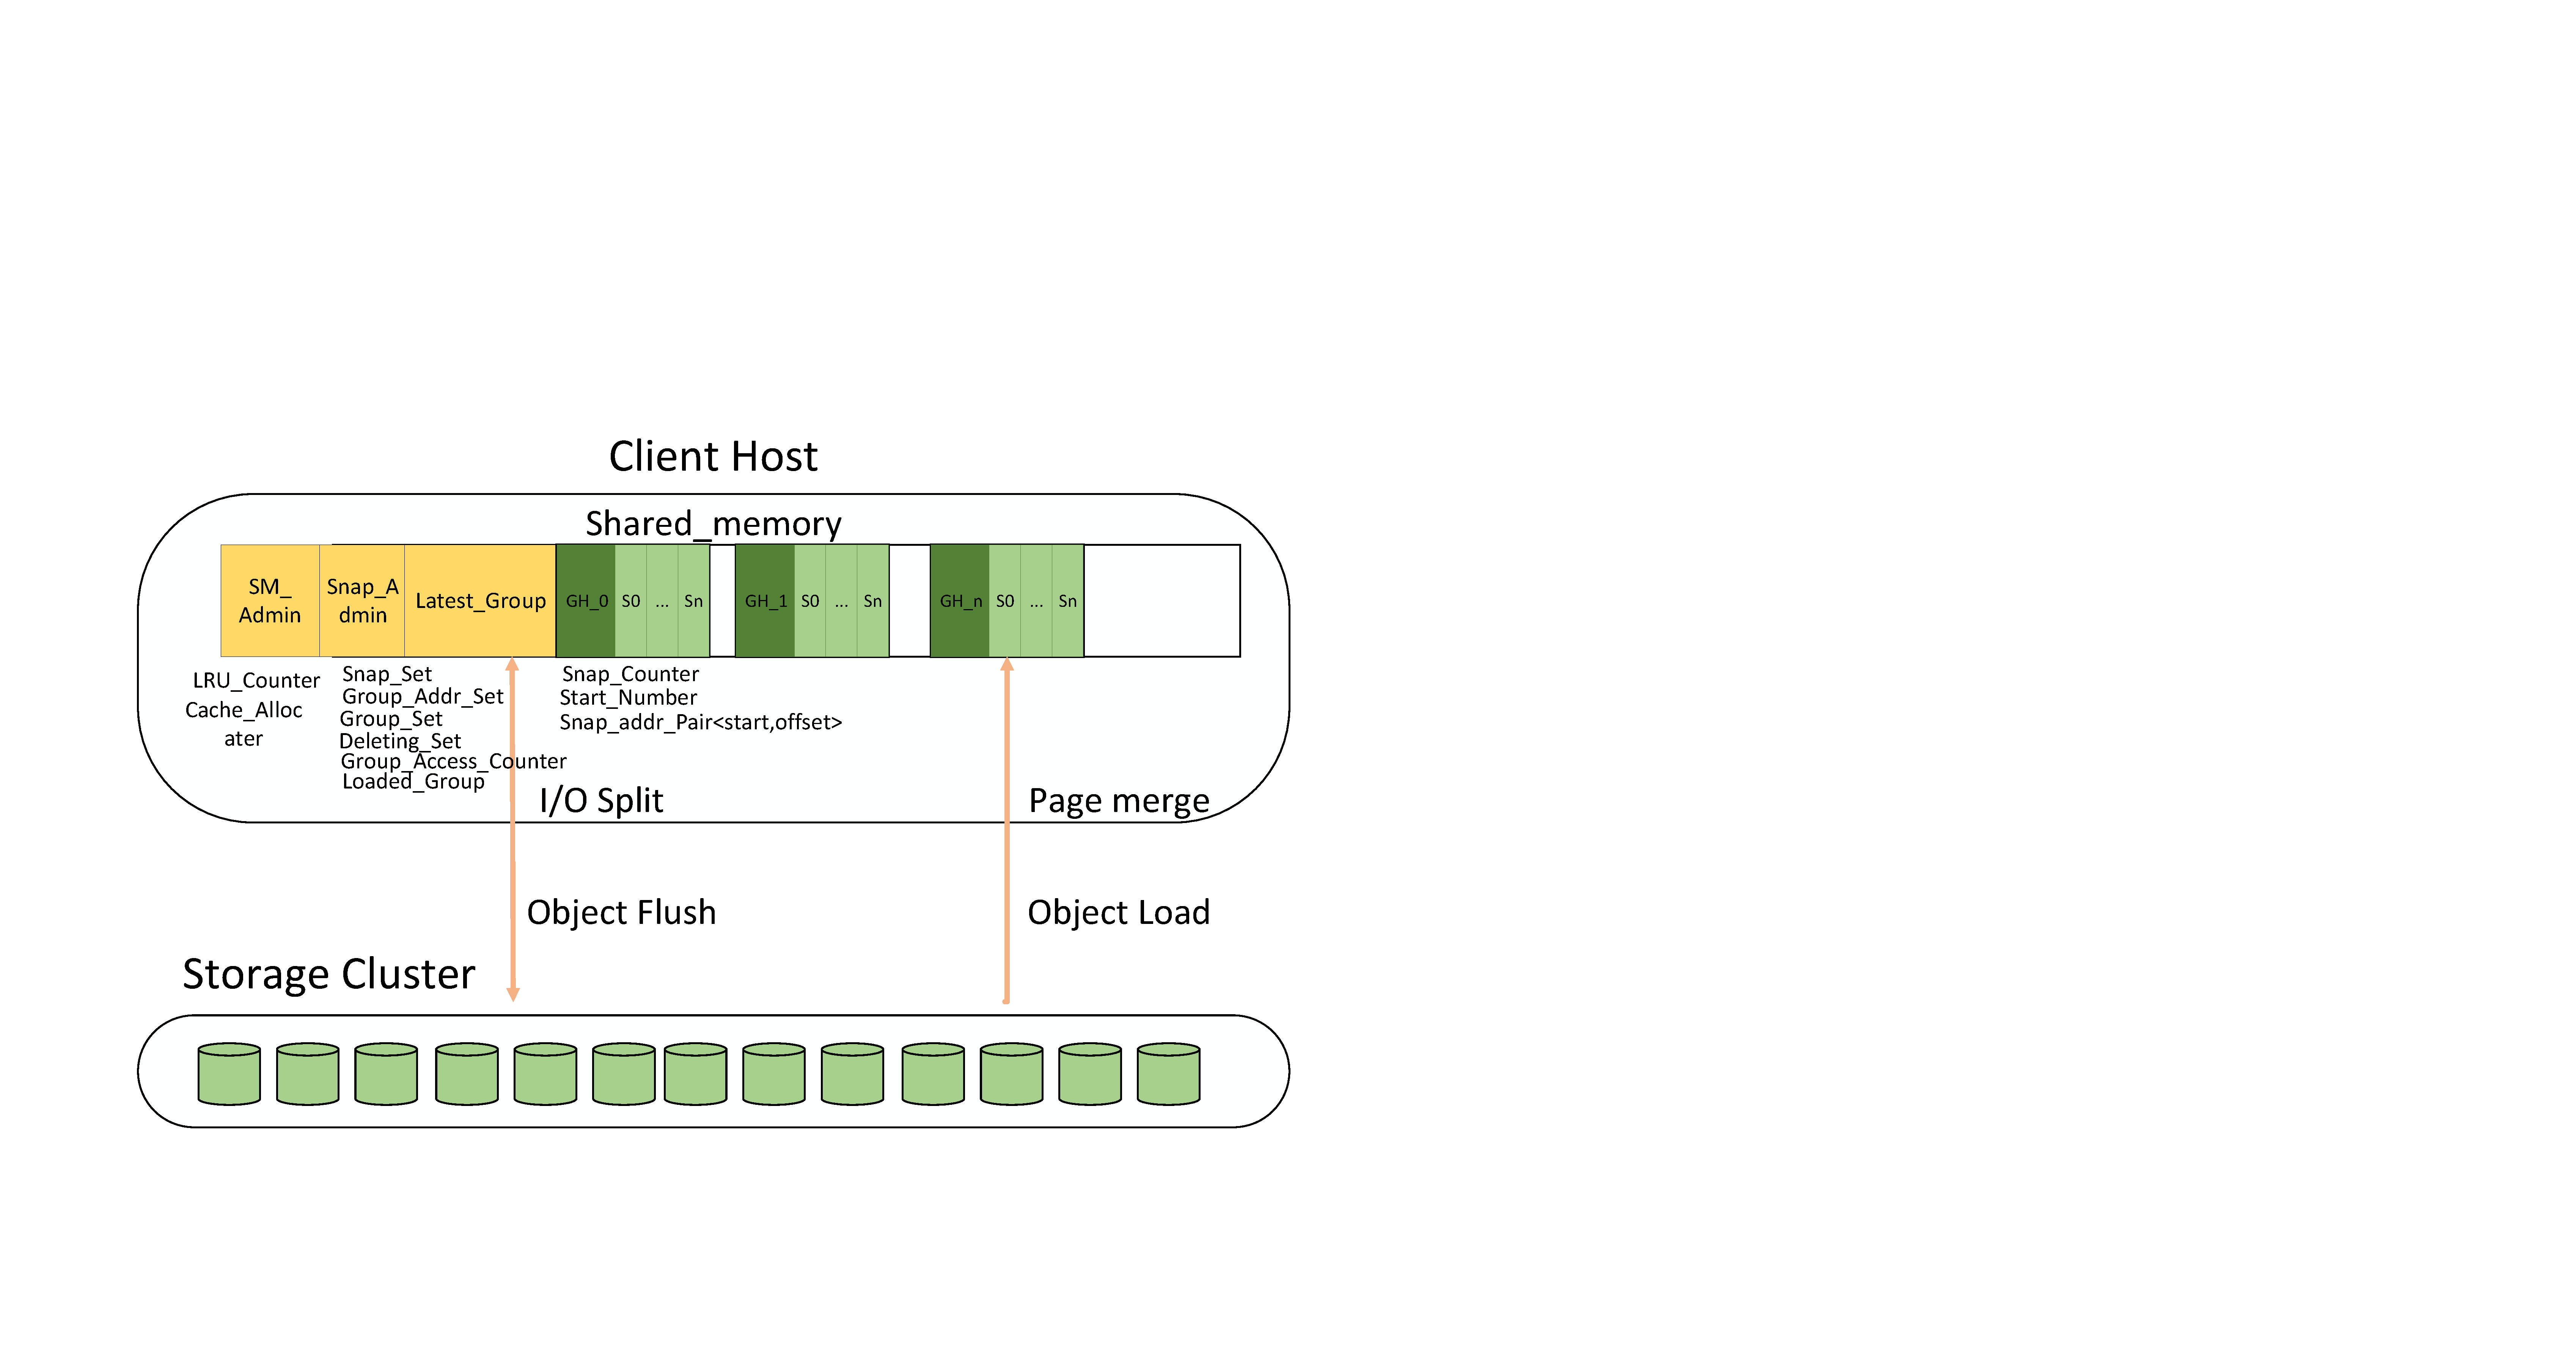
\includegraphics[width=\columnwidth]{figures/ceph_pic/cache_managment.pdf}
	\caption{Cache management of GSnap index on client host}
	\label{fig:cache_managment}
\end{figure}
\vspace{-0.3cm}

\subsection{GSnap Recovery Model and Analysis}
\label{section:Recovery model}
In this subsection, we theoretically analyze and compare GSnap with
the traditional and optimized indexes, abbreviated as T-index and
O-index, from two perspectives: the time cost of building an index and
the memory overhead. We also determine the number of snapshots $S$ and
the object budget $O$ based on the benefit.

When recovering and cloning a snapshot, the system loads snapshot
group and constructs the index in memory first. However, due to the
sharing of subtrees, the prerequisite for the construction of the
current snapshot tree is that all the subtrees in the group have been
constructed.  The dependence chain length of the group is a key factor
for snapshot recovery, to avoid loading indexes that do not be
accessed.  Further, the memory consumption of the group should be
cautious. The reason is that the memory of the system allocated by the
client node is limited.  Therefore, we compare the existing indexes
from these two perspectives respectively.

\begin{table}[htbp]
	\centering
	\caption{Group recovery notation definition.}
	\label{table:paramters}
	\resizebox{\columnwidth}{26mm}{
		\begin{tabular}{cc}
			\hline
			Notation & Description                                                  \\ \hline
			$D$        & The size of the block device (GB)                             \\ \hline
			$E$        & The object size of the block device (KB)                             \\ \hline
			$r$        & The longest snapshot interval with reference relationship                  \\ \hline
			%				$P$        & The average update ratio of snapshots                        \\ \hline
			$B$        & The network bandwidth of the storage cluster (Gbps)                 \\ \hline
			$T_a$        & The time cost of accessing memory, about 100 ns                         \\ \hline
			$T_r$       & The time cost of restoring a snapshot                                  \\ \hline
			$M_r$       & The memory overhead of restoring a snapshot                                 \\ \hline
			$M_c$       & The memory consumption of a compete tree                                 \\ \hline
			$M_p$       & The memory consumption of a partial tree                                 \\ \hline
			$T_t$       & The transmission time of each data block                     \\ \hline
			$T_i$       & The average time to insert a node in the snapshot index tree \\ \hline
			$T_l$       & The average time to locate a leaf node                         \\ \hline
			%				$O$       & The max number of modified objects in a group                          \\ \hline
			%				$S$       & The max number of snapshot in a group                        \\ \hline
		\end{tabular}
	}
\end{table}

\textbf{Time overhead.} Time overhead refers to the time span in which
snapshot could provide services when accessing a certain snapshot. At
the stage, the snapshot index is loaded into the memory and the data
blocks are still in the physical cluster. We ignore the latency of the
access request from the application layer. Even if the delay of the
T-index and O-index is higher than the GSnap in loop access
requests. We also limit the snapshot recovery to a group rather than
across groups for simplicity. So we have the following equation to
define the latency and memory overhead of restoring a snapshot. It may
consist of three parts: \textcircled{1} transform the index blocks
from the cluster to the client node; \textcircled{2} construct the
tree and insert the addresses of all data blocks; \textcircled{3}
locate all leaf nodes when coping nodes to construct a complete tree
from the former index. The respective latencies of the three stages
are:

\begin{small}
	\begin{equation}
	\begin{split}
	T_t&=\frac{1}{32 \times B} \\
	%		T_i > T_l&= O(\log_2(n))  \\
	T_i > T_l&= 8\times \log_2(\frac{D}{E})\times T_a \\
	\end{split}
	\end{equation}
\end{small}
\vspace{-0.2cm}

The O-index and GSnap contain traverse overhead because they may
construct the complete tree. The time overhead of those indexes during
the snapshot restoration is as follows:

\vspace{-0.2cm}
\begin{small}
	\begin{equation}
	\begin{split}
	T_r(T) &= \frac{D}{4}\times(r+1)\times T_t+ 256\times \frac{D}{E} \times p \times(r+1) \times T_i\\
	T_r(O) &= \frac{D}{4}\times T_t+ 256\times \frac{D}{E} \times (T_i + T_l)\\
	T_r(G) &= \frac{D}{4}\times(s)\times T_t+ 256\times \frac{D}{E} \times (1+(s -1)\times p) \times \\
	&	(n+1)\times T_i+ 256\times \frac{D}{E} \times T_l
	\end{split}
	\end{equation}
\end{small}
\vspace{-0.2cm}

Assume $B=D$, the insert overhead of the tree is 4 times the traversal overhead. Then:

\vspace{-0.2cm}
\begin{small}
	\begin{equation}
	\begin{split}
	%		T_r(T) &= \frac{D}{4}\times(n+1)\times T_t+ 256\times n \times p \times(n+1) \times T_i\\
	\frac{T_r(T)}{T_r(G)}\leq \frac{16\times(r+1)\times P}{16\times S +1}
	\end{split}
	\end{equation}
\end{small}
\vspace{-0.2cm}

\textbf{Memory overhead.} Memory overhead refers to the memory
consumption of constructing a snapshot index in the shared memory of
the client host. We measure the memory overhead of each index. When
the block device and the object size are fixed, the memory consumption
of the complete snapshot index is also fixed. The memory consumption
of the partial snapshot index is related to the update ratio. We
simply set $M_p = pM_c$ MB.  The memory overhead of different indexes
during the snapshot restoration are as follows:

\vspace{-0.2cm}
%A key aspect of the GSnap is memory efficient index. 
\begin{small}
	\begin{equation}
	\begin{split}
	M_r(T) &= (r+1) \times M_p\\
	M_r(O) &= M_c\\
	M_r(G) &= M_c + (S-1)\times M_p
	\end{split}
	\end{equation}
\end{small}
\vspace{-0.2cm}

Other snapshots with dependency are loaded in the T-index and GSnap,
so we only compare the average memory consumption of each snapshot
index. Obviously, compared with O-index, the memory overhead of GSnap
is effectively reduced:

\vspace{-0.2cm}
\begin{small}
	\begin{equation}
	\begin{split}
	\frac{M_r(O)}{M_r(G)} &= \frac{S}{1+(S-1)\times P}
	\end{split}
	\end{equation}
\end{small}
\vspace{-0.2cm}

\textbf{Balance load speed and memory consumption.} Both snapshot
index loading latency and memory consumption are tied to $S$ and
$P$. We comprehensively consider these parameters into loading speed
and memory overhead and establish different weights in the system to
satisfy the needs of snapshot recovery in various applications to
explore the maximum benefit. We set the benefit as $\Delta$, $\alpha$
and $\beta$ as the weights respectively. The benefit function is the
following:

\vspace{-0.2cm}
\begin{small}
	\begin{equation}
	%		M_r(T) &= \frac{S}{1+(S-1)\times P}
	\begin{split}
	\Delta = \alpha \times \frac{S-(1+(S-1)\times P)}{S}+\beta\times\frac{r+1-(S+\frac{1}{16\times p})}{r+1} 
	\end{split}
	\end{equation}
\end{small}
Assume $\alpha=\beta=0.5$, simplify and conclude that: when $S=\sqrt{(1+r)(1-P)}$, the benefit $\Delta$ gets the maximum.

The above analysis shows that grouping snapshot index could
effectively balance the recovery speed and memory usage, and
determines the group size by workload parameters, namely $r$ and $P$,
to achieve the max benefit.  However, in GSnap, to adapt to the
snapshot continuous access, and the subsequent group length is also
related to the snapshot update ratio and the average access length.
The $n$-th group size is set to: $O_n=\max(S_{n-1}^\ast, S_n^\ast)
\times P_{n-1}$.

\subsection{Snapshot Deleting and Index Merging}
To save the storage of the cluster, the system deletes historical
snapshots with different lengths instead of simply deleting in
batches. The system deletes snapshots based on their
importance. Snapshots with low weight are more likely to be
deleted. Earlier snapshots are less important. At the same time,
snapshots taken at the critical timing are retained. This creates
snapshots sets of varying degrees of sparseness.

\textbf{Deleting snapshot.} Deleting a snapshot is divided into two
parts. The first is to delete the data blocks contained in the
snapshot, and the second is to modify the index of the snapshot.  The
data block of the snapshot is removed once it is not referred by other
snapshots, that is, $Block\_Reference$ is equal to 0. Otherwise the
reference is reduced by one.  The system checks the group whether is
in the $GS$ to locate the address of the target index, then traverses
all leaf nodes and decreases the number of updates
$Current\_Group\_Update\_Counter$ for the current group by 1. When the
traversal is completed, if the index has no child nodes, the group
deletes the head node of the index, and decreases the number of
snapshots in the group. Otherwise GSnap sets the index invalid in the
group. Deleting the snapshot set needs to record the set to avoid an
invalid merge operation. the thread tags the set in $Deleting\_Set$,
and clears the record when the snapshot set is deleted.

\textbf{Merging index between groups.} The index in the group is also
removed after the snapshot is deleted. However, the memory assigned to
this group is fixed, the group should be merged when the most of
snapshots are deleted to reclaim the memory and improve snapshot
recovery.  For simplicity, snapshot merges are performed only between
adjacent snapshot groups, which integrates the snapshot indexes of the
latter group into the former group. So the condition of merging groups
is that the free space of the former snapshot group could contain the
latter group. In the latter group, only the first one is the complete
snapshot tree, and the following snapshot indexes are partial snapshot
trees. Thus the first complete snapshot tree in the latter group needs
to be traversed, to rebuild as the partial snapshot tree in the former
group. However, subsequent partial snapshot trees depend on the
original complete snapshot tree, so all partial snapshot trees need to
be regenerated in the first group. Specially, the merge process checks
whether the groups to be merged are in $Deleting\_Set$, and if so, it
skips the merge operation and waits for the deletion. Then the process
traverses all the leaf nodes of the partial snapshot tree in order,
and regenerates the partial snapshot tree points to the snapshot tree
in the former group.

\subsection{Snapshot Interval Analysis of Merging Group}

In the process of merging group, the leave nodes of all snapshots of
the latter group are traversed, so the number of snapshots and the
update ratio affect the merge efficiency. The benefit of merging
groups is primarily accelerating snapshot recovery because only the
required groups need to be loaded and no additional groups. At the
same time, the memory utilization is improved. The number of partial
snapshots in the latter group is the key factor when merging
groups. Although the merge efficiency is improved if the number is
tiny, there are a large number of internal fragments in the group
before triggering the merge operation, which hinders the snapshot
recovery and memory utilization. So we theoretically analyze the
appropriate length of the latter group when merging.

\begin{table}[htbp]
	\centering
	\caption{Group merging notation definition.}
	\label{table:mergegroupparamters}
	\resizebox{\columnwidth}{16mm}{
		\begin{tabular}{cc}
			\hline
			Notation & Description                                                  \\ \hline
			$k$       & The number of partial snapshots in the latter group              \\ \hline
			%				$L_c$      & The average consecutively accessed snapshot set interval                     \\ \hline
			$B_o$    & The average bytes of the nodes occupied by data block             \\ \hline
			$T_n$        & the average node generation delay for one block                         \\ \hline
			$T_d$       & Disk I/O latency             \\ \hline
			$T_n$       & Network I/O latency                   \\ \hline
			$B_d$       & Disk I/O block size             \\ \hline
			$B_n$       & Network I/O block size                   \\ \hline
			
		\end{tabular}
	}
\end{table}

\textbf{Merging overhead.}  Traversing the complete tree is required
for the merging operation, while traversing the partial tree is
optional. So the number of subsequent partial trees determines the
latency of the merge operation.  The merge overhead is determined by
the number of partial indexes in the latter group, the average update
ratio of snapshots, and the average node generation delay.

\vspace{-0.2cm}
\begin{small}
	\begin{equation}
	\label{overhead}
	\begin{split}
	Overhead&= k\times P \times T_n
	\end{split}
	\end{equation}	
\end{small}
\vspace{-0.2cm}

\textbf{Merging benefit.} The benefit of merging operation consists of
two parts. The first is to reclaim the memory space of the latter
group, and the second is that only the target group which needs to be
loaded without additional groups during snapshot recovery. Recycling
the index could reduce the frequency of swapping out groups when the
shared memory is fixed. We consider swapping out the group to disk as
the main factor, and the first benefit of the merging operation is
measured by the delay of swapping out the group.  The recovery process
loads at least one less group into the client node once the groups are
merged from the storage cluster, and the second benefit of the merging
operation is measured by the delay of loading group. We consider
loading process only reduces one group and the delay is mainly network
overhead.

\vspace{-0.3cm}
\begin{small}
	\begin{equation}
	\label{benefit}
	\begin{split}
	Benefit&= P\times L_c \times B_o \times(\frac{T_d}{B_d} + \frac{T_n}{B_n})
	\end{split}
	\end{equation}
\end{small}
\vspace{-0.4cm}

Calculated by formulas \ref{overhead} and \ref{benefit}, Merging
snapshot group only benefits when $k<=\frac{L_c\times B_o
  \times(\frac{T_d}{B_d} + \frac{T_n}{B_n})}{T_n}$. So the merging of
groups does not wait until only the complete snapshot tree remains and
reduces the internal fragmentation of the group. Before the group
merging, it first checks whether the counter of snapshots $k$ in the
latter group meets the condition, and then determine whether the space
in the former group could accommodate the latter group. According to
the experimental configuration in Section \ref{Evaluation}, the value
of k is set $\frac{L_c}{5}$.

{\tiny {\normalsize }}
\section{Evaluation}
\label{Evaluation}
We perform our experiments on a Ceph cluster with 4 cloud elastic
compute services (ECS) running on Centos 7.9. Each ECS is equipped an
Intel Xeon 2.5GHz processor with 32 cores, 32GB memory and 256GB SATA
Disk and internal network bandwidth up to 10Gbps. The cluster
configures a OSD node and a Monitor node on three hosts respectively,
and the remaining host deploys a Ceph cluster client.  In our
evaluation, we built a GSnap index Embedded in Ceph v15.2.5. To
comprehensively evaluate our design, we also embedded the T-index and
O-index in the same version.  We create block devices of different
sizes through Ceph RBD interface, and then mount the block device on
the client node. Besides we create the XFS file system on the block
device, and deploy the database.  We use MySQL 5.7 with InnoDB storage
engine and running TPC-C benchmark. We use the TPC-C because it is a
standard decision support benchmark with a well-known schema
consisting of familiar tables. We run the all types of transactions in
the benchmark. We report the Transactions Per Seconds (TPS) measured
at the client node. For the MySQL/InnoDB configuration, we set the
buffer pool as 1 GB and enable the direct I/O mode (O\_DIRECT) to
avoid the effect of file system page caching.  All experimental
results are the average value of 5 runs.

We create the Ceph client account on the client node as the administer
and create block devices in a pool which supports three replicas by
default. We configure block devices and their snapshots in the same
pool to reduce the block migration.  The size of the block device is
4GB by default and the punish factor $p$ set as 3/4.  Mysql is hosted
on the XFS file system and default set to 4KB page size, which we did
not change. We set the default disk I/O block size to 4KB and network
I/O block size to 1MB.


\subsection{Database Throughput}
The system takes snapshot periodically in the initial phase before
starting the TPCC \cite{Tpcc} benchmark, and the time cost of creating
a index is measured by the initial latency, which excludes the warm
time of the benchmark and the time of the mount operation. Then we run
the benchmark for 200 seconds in the snapshot period. For the
convenience of evaluation, we do not delete snapshots.

To understand the performance of GSnap under database workloads, we
evaluate the throughput on the various degrees of the connections with
the other indexes. We do not perform snapshot recovery operations when
creating snapshots, in order to reduce the shared memory usage. At the
same time, when the snapshot group is completed, the group index is
actively loaded into the remote storage cluster. We use the default
script to create the database index and set the number of the database
warehouses to 20. Specially, we adjust the connection of database to
model the workloads.

\begin{figure}[htbp]
	\centering
	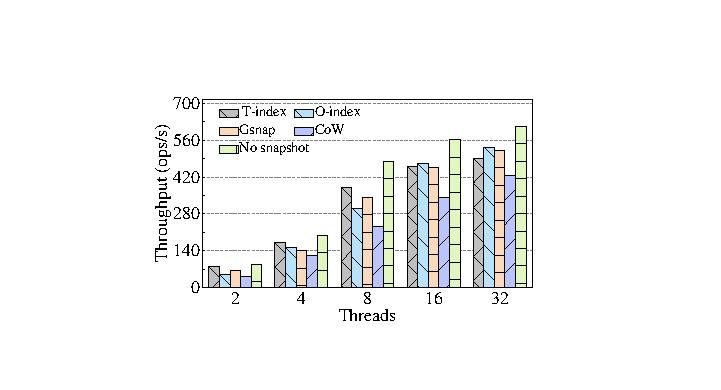
\includegraphics[width=0.7\columnwidth]{figures/ceph_pic/eval_overview.pdf}
	\vspace{-0.4cm}
	\caption{Throughput }
	\label{fig:databasethroughput}
\end{figure}


As shown in Figure \ref{fig:databasethroughput}, GSnap outperforms the
O-index for database workloads. The reason is that GSnap reduces the
number of nodes, when the file system writes a new data block, Gsnap
could directly look up the index to locate the target data block,
while O-index needs to generate a node and then process it.  But as
the number of threads increases, the times of writing data blocks
increases, and the nodes of the tree tend to be saturated, so O-index
and GSnap are basically the same in index locating cost, so the number
of transactions they process is also close. GSnap is lower than
No-snapshot by 9\%. The reason is that the copy operation of the data
block is reduced in RoW, but the snapshot still copies the uncovered
data to the current object. The transaction throughput is affected by
the database workload. We discuss the read/write ratio on snapshot
performance in Section \ref{IPerforamce}.

\subsection{Snapshot Group Length}
In this subsection we discuss the impact of snapshot group length on
snapshot recovery. Since the snapshot update ratio and the average
snapshot access length determine the length of the latter group, we
fix the parameters and only measure the impact of the snapshot length
on snapshot recovery. We create 100 snapshots to evaluate snapshot
recovery and then randomly recovered a snapshot group. The benefits of
GSnap compared to other indexes are highlighted by statistical
recovery latency and memory overhead.

\begin{figure}[htbp]
	\centering
	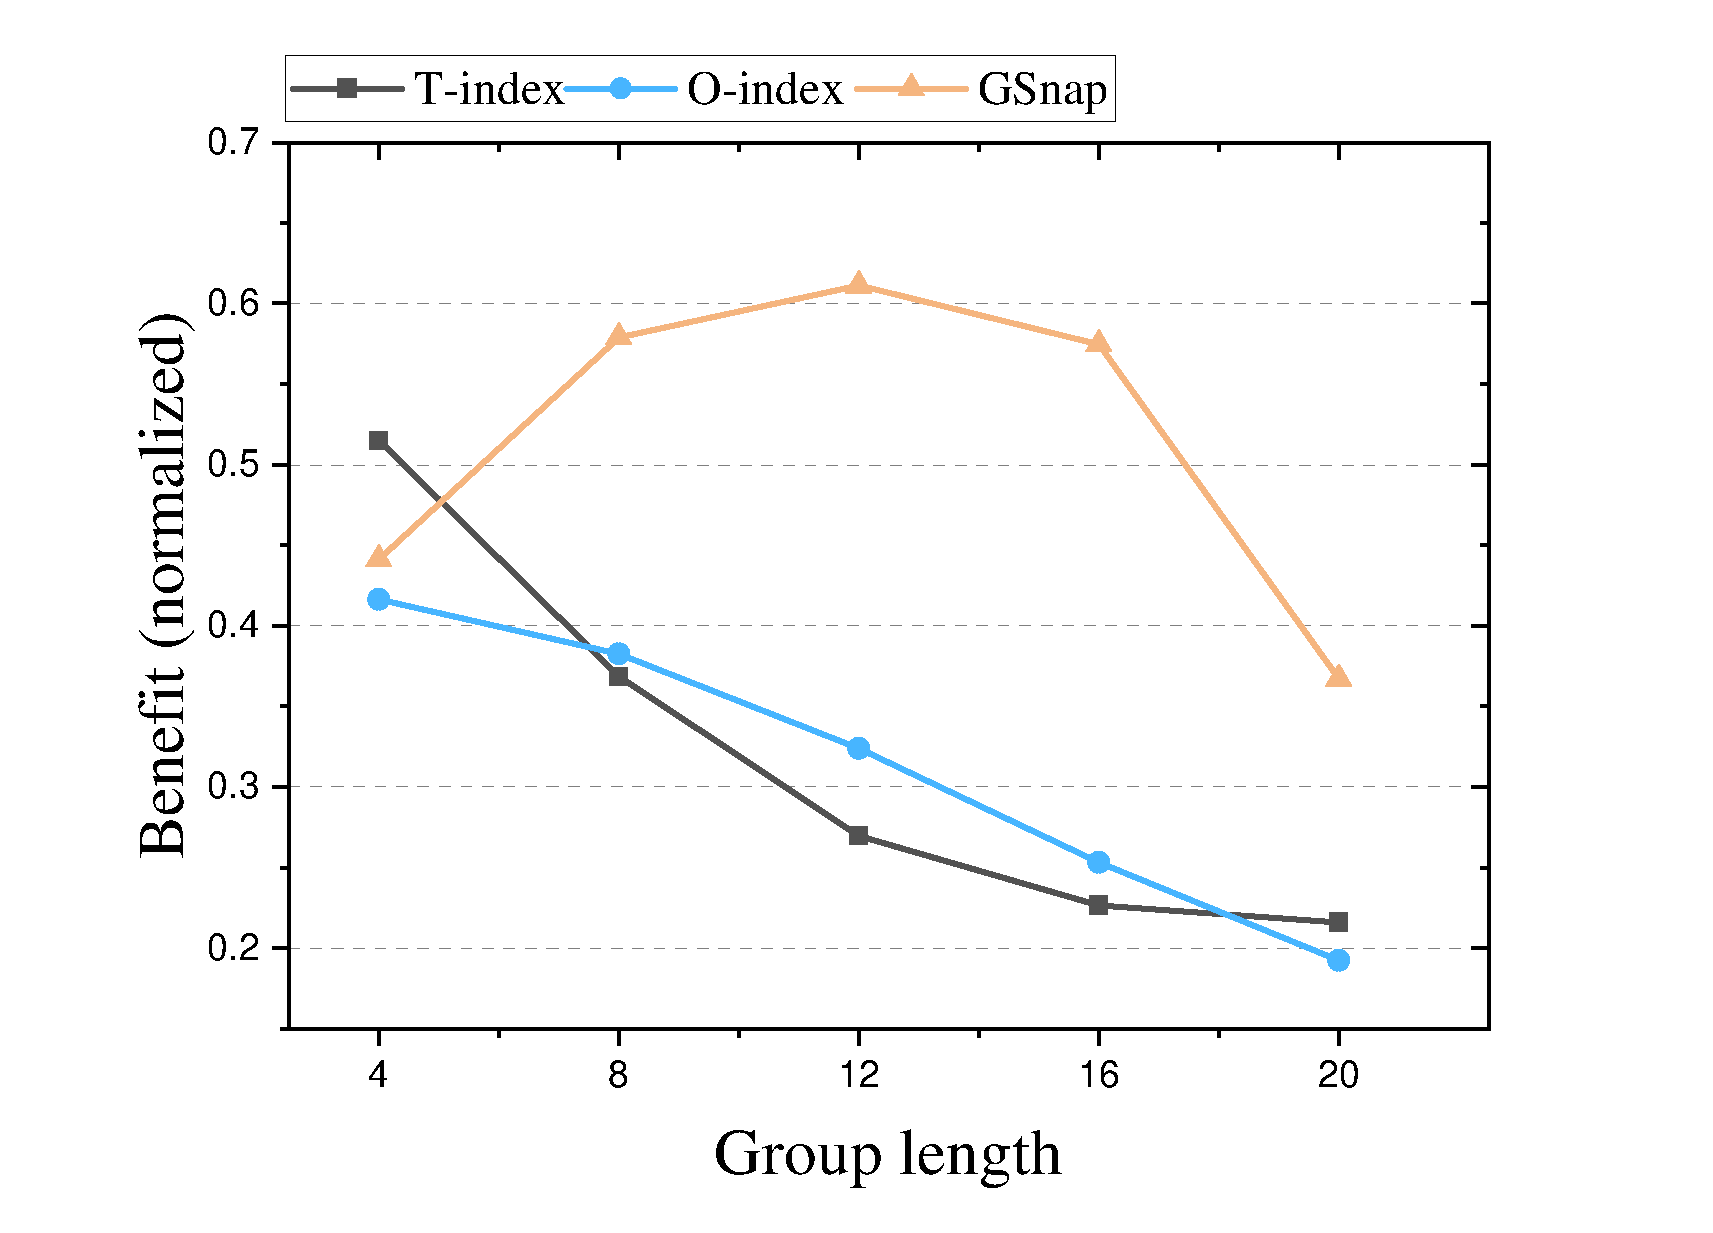
\includegraphics[width=0.6\columnwidth]{figures/ceph_pic/eval_grouplength.pdf}
	\vspace{-0.4cm}
	\caption{The benefit to restore a single snapshot group}
	\label{fig:grouplength}
	
\end{figure}

As shown in Figure \ref{fig:grouplength}, GSnap cuts off snapshot
references and shares child nodes within the group, which makes its
revenue higher than both T-index and O-index. Because of the snapshot
dependency, T-index loads its dependent snapshot indexes when
restoring the snapshot collection, and in fact, the memory usage of
the group is related to the length of the dependency chain. The
performance of O-index degrades as the length of the snapshot set
increases, because each index is a complete snapshot tree. GSnap has
the largest profit when the snapshot group length is 12, which is
close to the optimal value in the theoretical analysis. As the
snapshot length increases, the number of snapshots that need to be
loaded and the index memory increase, resulting in lower benefits, but
higher than other indexes.

\subsection{Snapshot Recovery}
Before evaluating snapshot recovery, we clone all snapshots because
snapshots are read-only and flush the group index out the shared
memory on the client node, which ensures that the group index is
loaded from the storage cluster when restoring the snapshot. The
snapshots are not deleted when restoring process. There are two types
of application scenarios for accessing snapshots: single snapshot and
snapshot set.  Therefore, we separately evaluate the recovery
performance of those indexes in the two scenarios.  We fix the length
of snapshot group to 20 since the length of the snapshot group affect
the snapshot recovery.

\begin{figure}[htbp]
	\centering
	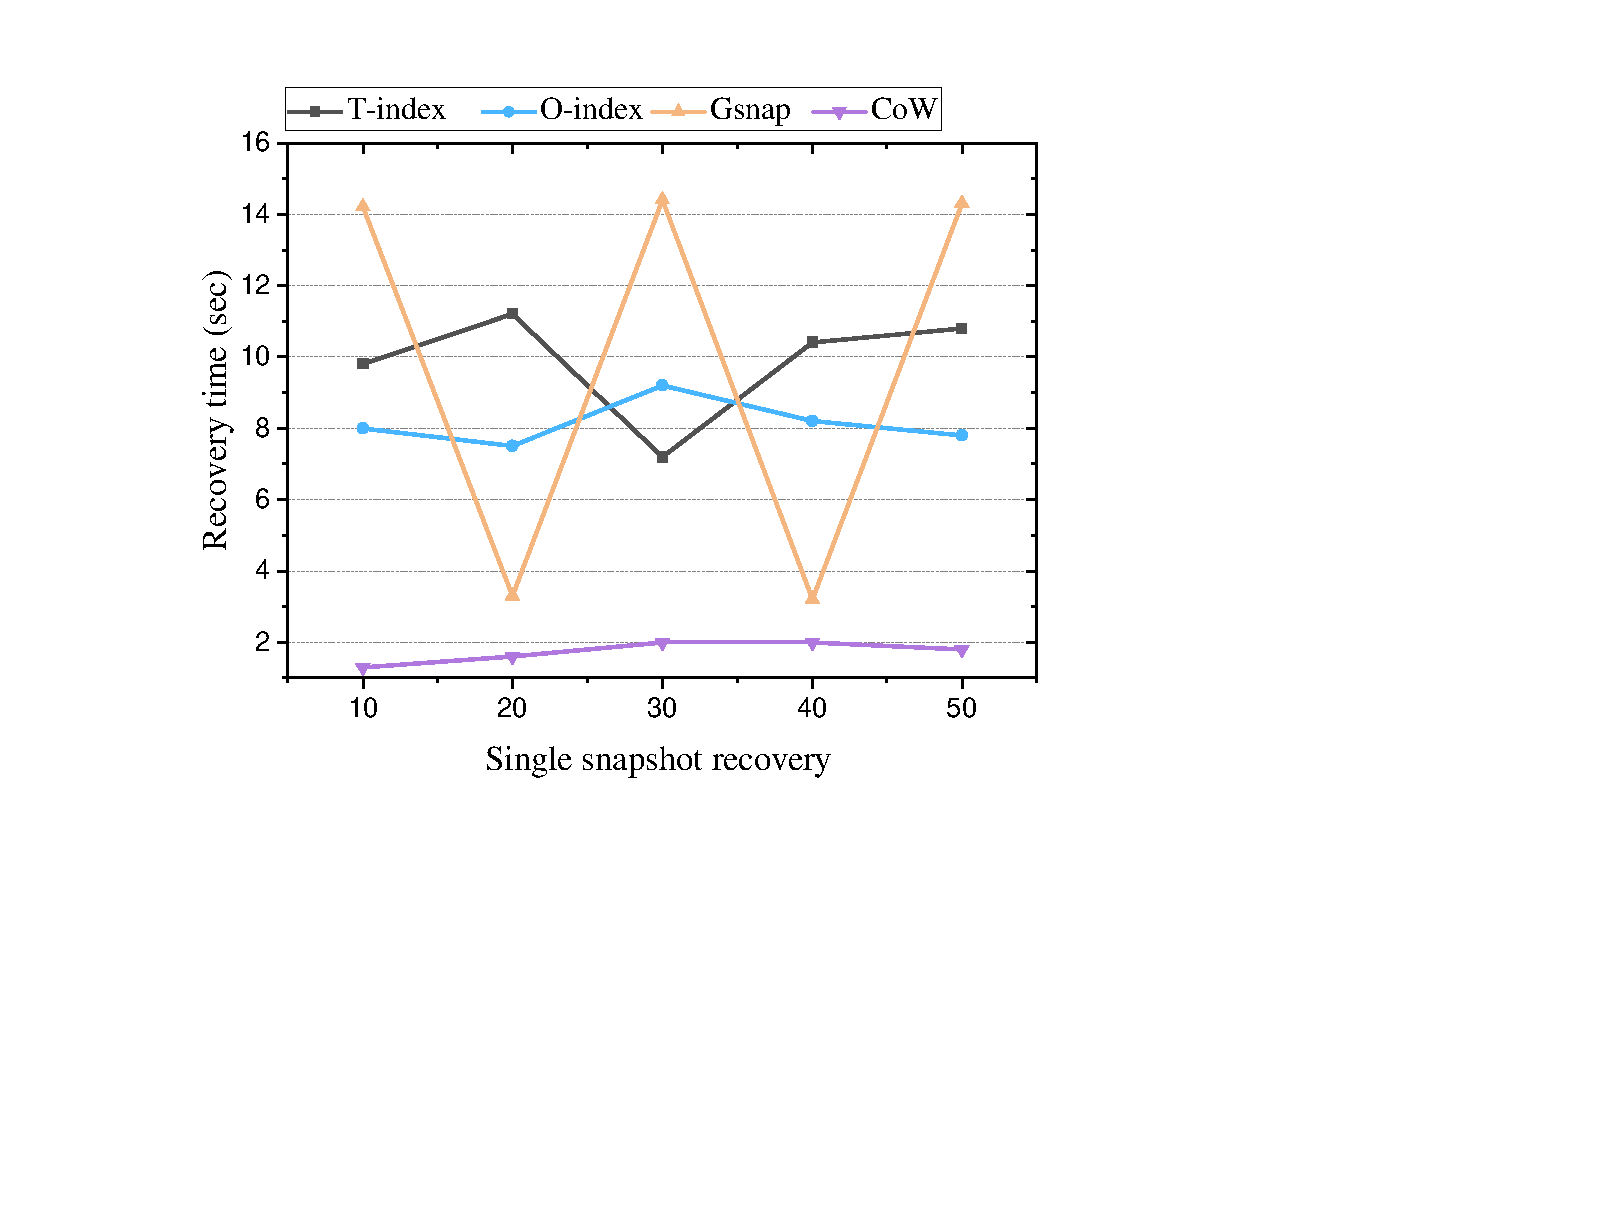
\includegraphics[width=0.6\columnwidth]{figures/ceph_pic/eval_point.pdf}
	\vspace{-0.4cm}
	\caption{The latency to restore a single snapshot}
	\label{fig:snapshotpoint}
\end{figure}


The recovery snapshot interval is set to 10, the purpose is to prevent
the recovery of a single snapshot from evolving into the recovery of a
snapshot collection and the snapshots are recovered in order. As shown
in Figure \ref{fig:snapshotpoint}, we set up to restore the snapshots
sequentially, so the snapshot indexes that the latter restored
snapshots depend on have been loaded into shared memory.  For GSnap,
if the snapshot to be restored is already in the loaded group, the
recovery latency is low, such as restoring the snapshots 20 and 40.
But the recovery delay of GSnap exceeds O-index, the reason is that
GSnap needs to load more indexes than O-index.  All indexes in the
group are loaded when GSnap restores a single snapshot, while O-index
only needs to restore one snapshot index.

\vspace{-0.3cm}
\begin{figure}[htbp]
	\centering
	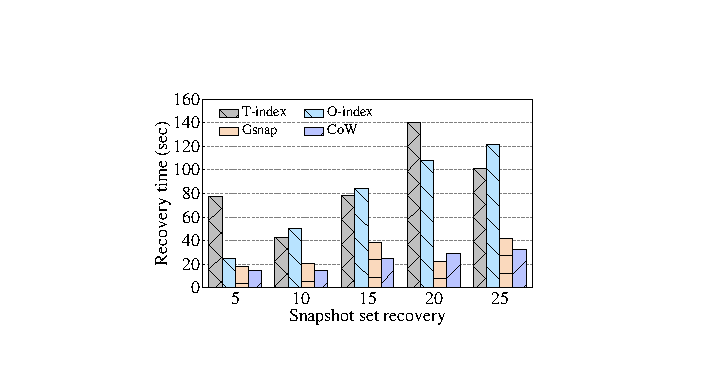
\includegraphics[width=0.7\columnwidth]{figures/ceph_pic/eval_sequence.pdf}
	\vspace{-0.4cm}
	\caption{The throughput to restore snapshot set}
	\label{fig:snapshotlength}
	
\end{figure}
\vspace{-0.2cm}

We evaluate the delay of restoring snapshot sets of different lengths,
to simulate continuous access to snapshots. We set all snapshot sets
to randomly restore from the groups, and refresh the shared memory
after each recovery operation to ensure the latency accuracy.  As
shown in Figure \ref{fig:snapshotlength}, compared with O-index, the
speedup of GSnap is up to 79\%, because in the loaded snapshot
indexes, only 2 indexes are complete snapshot trees, and the others
are partial snapshot trees, which can effectively reduce the index
size of the transfer process.  The recovery time of T-index
deteriorates when restoring 20 snapshots, the reason is that the
serial number of the first snapshot in recovery set is 34 and the
dependency length of T-index is long.


\subsection{Snapshot Deleting}
In order to keep the number of snapshots constant, the system
continuously deletes snapshots sparsely. We evaluate the latency of
deleting snapshot sets of different lengths to keep the important
snapshots. Besides, we also measure the overhead of merging the
groups.  Since CoW does not depend on previous snapshots, we only
compare O-index, T-index and GSnap.

\begin{figure}[htbp]
	\centering
	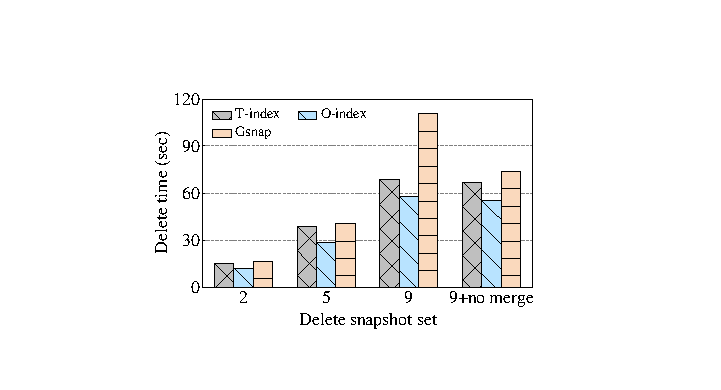
\includegraphics[width=0.7\columnwidth]{figures/ceph_pic/eval_delete.pdf}
	\vspace{-0.4cm}
	\caption{The latency to delete snapshot set}
	\label{fig:delete}
	\vspace{-0.4cm}
\end{figure}

As shown in Figure \ref{fig:delete}, when GSnap deletes snapshots, the
latency is close to T-index when the snapshot length is short, only
higher than 8\%. This is because when GSnap deletes an index, it needs
to traverse all leaf nodes to determine whether the data block can be
deleted. We add an additional set of snapshot delete operation for the
unmerged group, and merge operations degraded performance by only
26\%. The reason is that 11 partial trees are left in the second group
that triggered the merge operation, which increases the traversal
overhead. The time of snapshot deletion is longer than GSnap due to
the data merge and the index deletions operations.  However, this cost
makes the largest benefits to the performance of critical snapshot
operations.  First, the efficient snapshot creation operations make a
small impact on its applications, thereby maintaining business
continuity in a cloud computing environment. Second, the frequency of
snapshot creation is much higher than the frequency of snapshot
deletion.

\subsection{Object Size}
In this subsection, we evaluate the impact of different object sizes
on index overhead and counter the proportion of the actual write size
in the data block.  Under the RoW mechanism, if the object is not
fully written, the uncovered data needs to be copied from the previous
snapshot to the current snapshot state. We set a balanced read-write
ratio because this value affects the saturation of the snapshot index.
We create 10 groups and randomly load snapshot groups, T-index and
O-index load the corresponding snapshot sets. Finally we evaluate the
memory consumption of the indexes.

\begin{figure}[htbp]
	\centering
	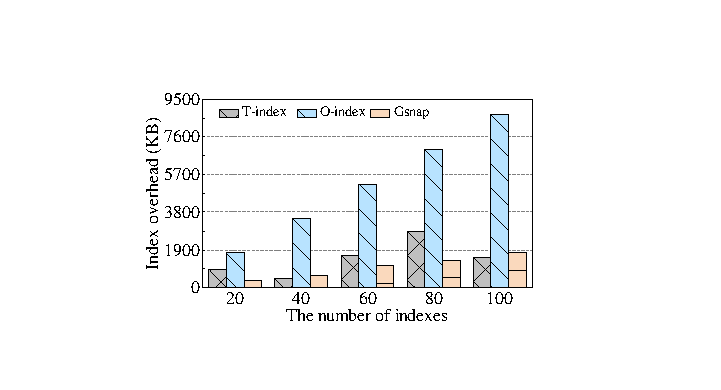
\includegraphics[width=0.7\columnwidth]{figures/ceph_pic/eval_indexmemory.pdf}
	\vspace{-0.4cm}
	\caption{The index overhead of snapshot}
	\label{fig:objectsize}
	\vspace{-0.3cm}
\end{figure}


As shown in Figure \ref{fig:objectsize}, the index overhead of O-index
exceeds that of GSnap, even though the number of the object decreases
as the size increases. The reason is that O-index is the complete
snapshot tree, whereas in Gsnap, only the first index within the group
is a complete snapshot tree, and the remaining indexes are partial
snapshot trees. the design of the group dilutes the average number of
nodes. The index overhead of GSnap is only 8\% higher than that of
T-index because the average indexing overhead is diluted by other
partial indexes within the group.  As the object size increases, the
actual data write ratio decreases. The reason is that at the end of
the snapshot, the system checks the coverage area of all objects and
copies the default content from the previous objects to the current
object.

\subsection{Merge Length}
In this subsection, we evaluate the effect of numbers of indexes in
the latter group in the merge operation. Likewise, we set the length
of the snapshot group to 20, and the recovered snapshot collection to
10. We randomly restore the set of snapshots to avoid trapping in a
single group.

As shown in Figure \ref{fig:merge}, the merge overhead increases with
the number of partial snapshots in the second group, because each
index needs to be traversed and merged into the previous group.  We
evaluate load delay reduction of 28.7 seconds for one group, which is
the benefit time of merging group. This delay is higher than the merge
overhead when the number of the partial tree is 5 in the latter group,
which means that the merge is only profitable at this time. The
snapshot group length is related to the average access length, so the
number of partial snapshots in the second group also dynamically
adapts to user access behavior when merging groups. As shown in Figure
\ref{fig:merge_recovery}, the more partial snapshots left when the
merge operation is initiated in the second group, the lower the
recovery latency. The reason is that most of the groups have been
merged and the snapshots within the group are saturated, so only one
group is restored. When there are 1 or 5 partial indexes in the group,
merge operations are reduced. Thus the collection needs to restore two
groups leading to increasing recovery overhead.

%\vspace{-0.3cm}
%\begin{figure}[htbp]
%	\centering
%	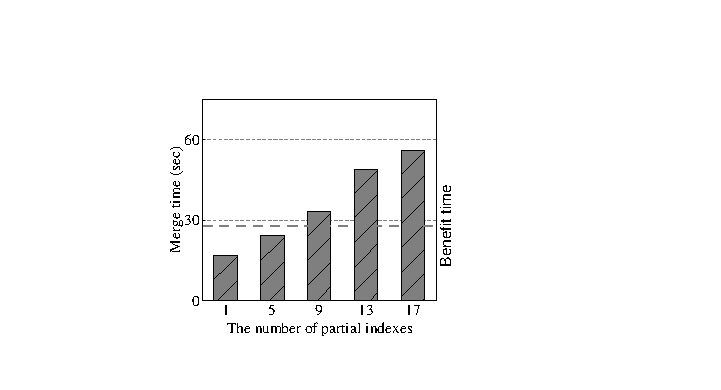
\includegraphics[width=0.8\columnwidth]{figures/ceph_pic/eval_merge.pdf}
%	\caption{The latency to delete snapshot set}
%	\label{fig:merge}
%\end{figure}
%\vspace{-0.3cm}
%
%\vspace{-0.3cm}
%\begin{figure}[htbp]
%	\centering
%	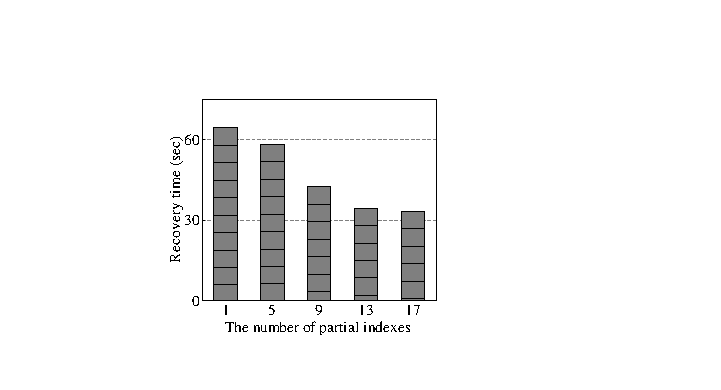
\includegraphics[width=0.8\columnwidth]{figures/ceph_pic/eval_merge_recovery.pdf}
%	\caption{The latency to delete snapshot set}
%	\label{fig:merge_rec}
%\end{figure}
%\vspace{-0.3cm}


%\begin{figure}[htbp]
%	\centering
%	\subfigure[Write-Only]{
%		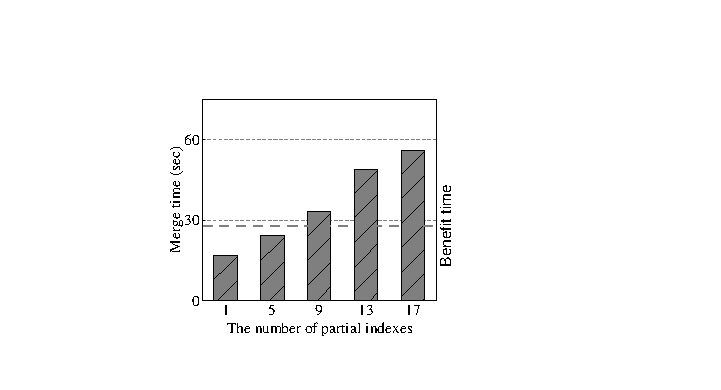
\includegraphics[width=0.5\columnwidth]{figures/ceph_pic/eval_merge.pdf}
%		\label{read-only}}
%	\subfigure[Balanced]{
%		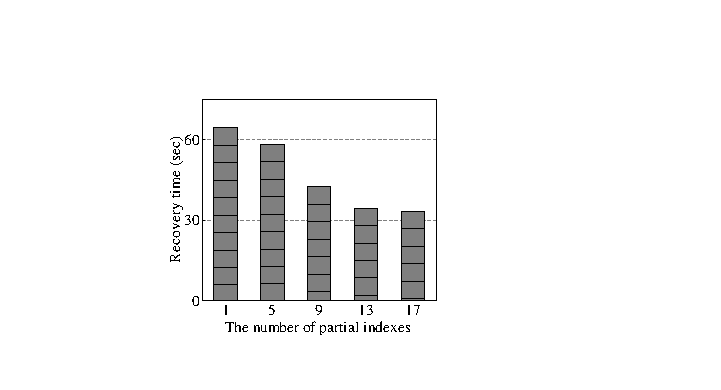
\includegraphics[width=0.5\columnwidth]{figures/ceph_pic/eval_merge_recovery.pdf}
%		\label{banlanced}}
%	\caption{The I/O performance for GSnap}
%	\label{fig:IO_performance}
%\end{figure}
\begin{figure}[htbp]
	\begin{minipage}[t]{0.45\linewidth}
		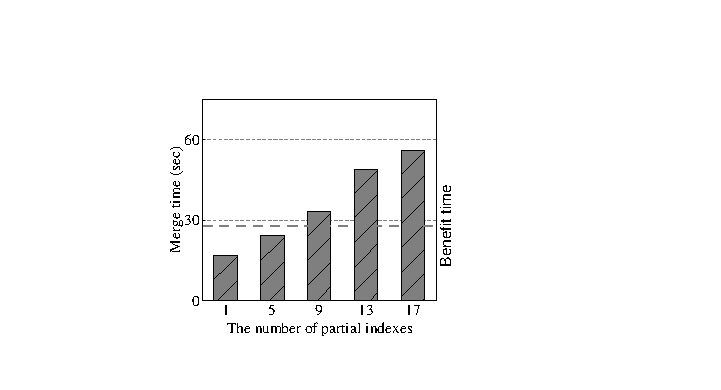
\includegraphics[width=\linewidth]{figures/ceph_pic/eval_merge.pdf} 
		\caption{The latency of recovering snapshot set} 
		\label{fig:merge}
	\end{minipage}%
	\hfill%
	\begin{minipage}[t]{0.45\linewidth}
		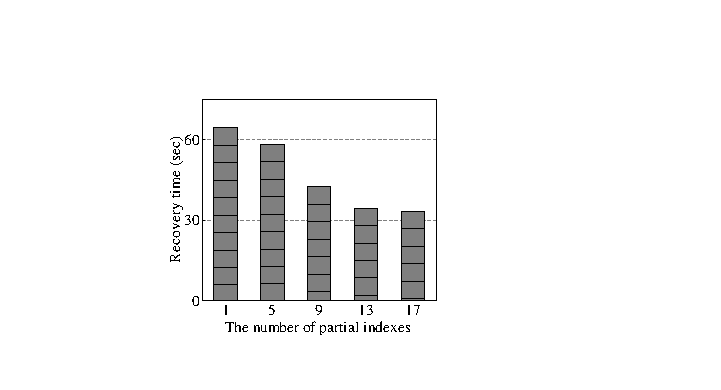
\includegraphics[width=\linewidth]{figures/ceph_pic/eval_merge_recovery.pdf}
		\caption{The latency of merging groups}
		\label{fig:merge_recovery}
	\end{minipage} 
\end{figure}

\vspace{-0.4cm}

\subsection{I/O Performance}


\begin{figure*}[htbp]
	\centering
	\subfigure[Write-Only]{
		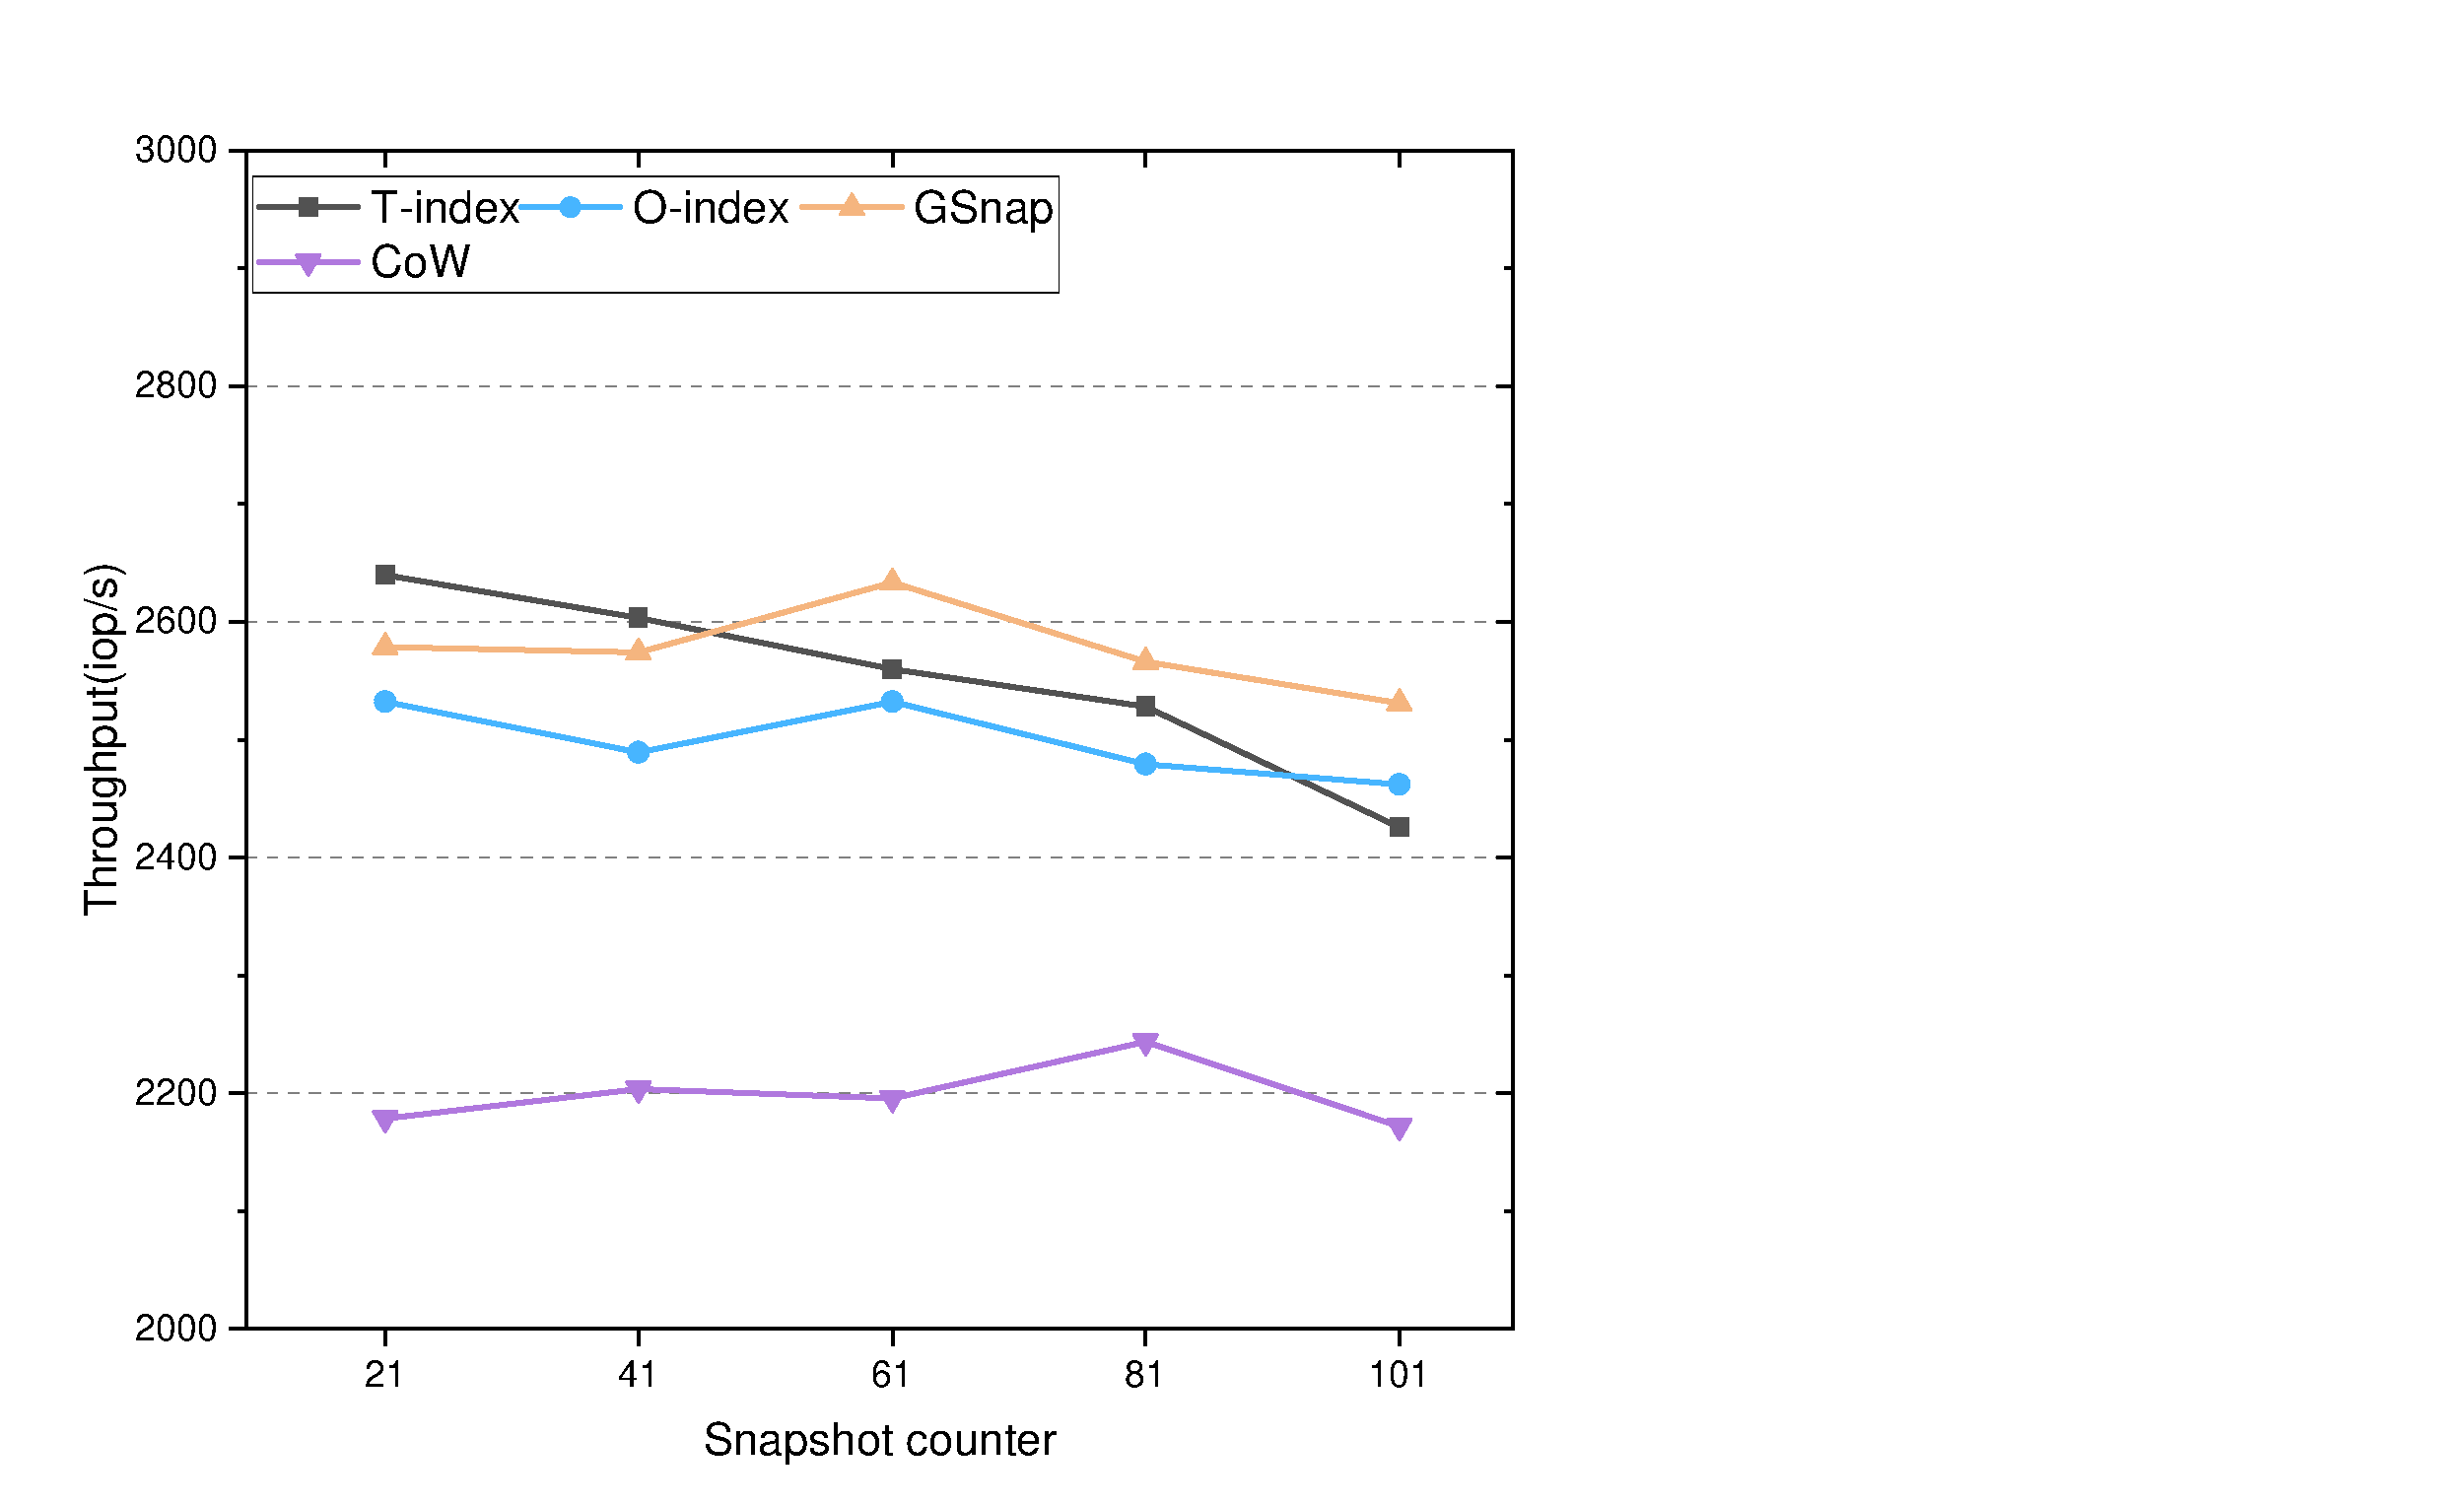
\includegraphics[width=6cm]{figures/ceph_pic/eval_write.pdf}
		\label{read-only}}
	\hspace{-5in}
	\subfigure[Balanced]{
		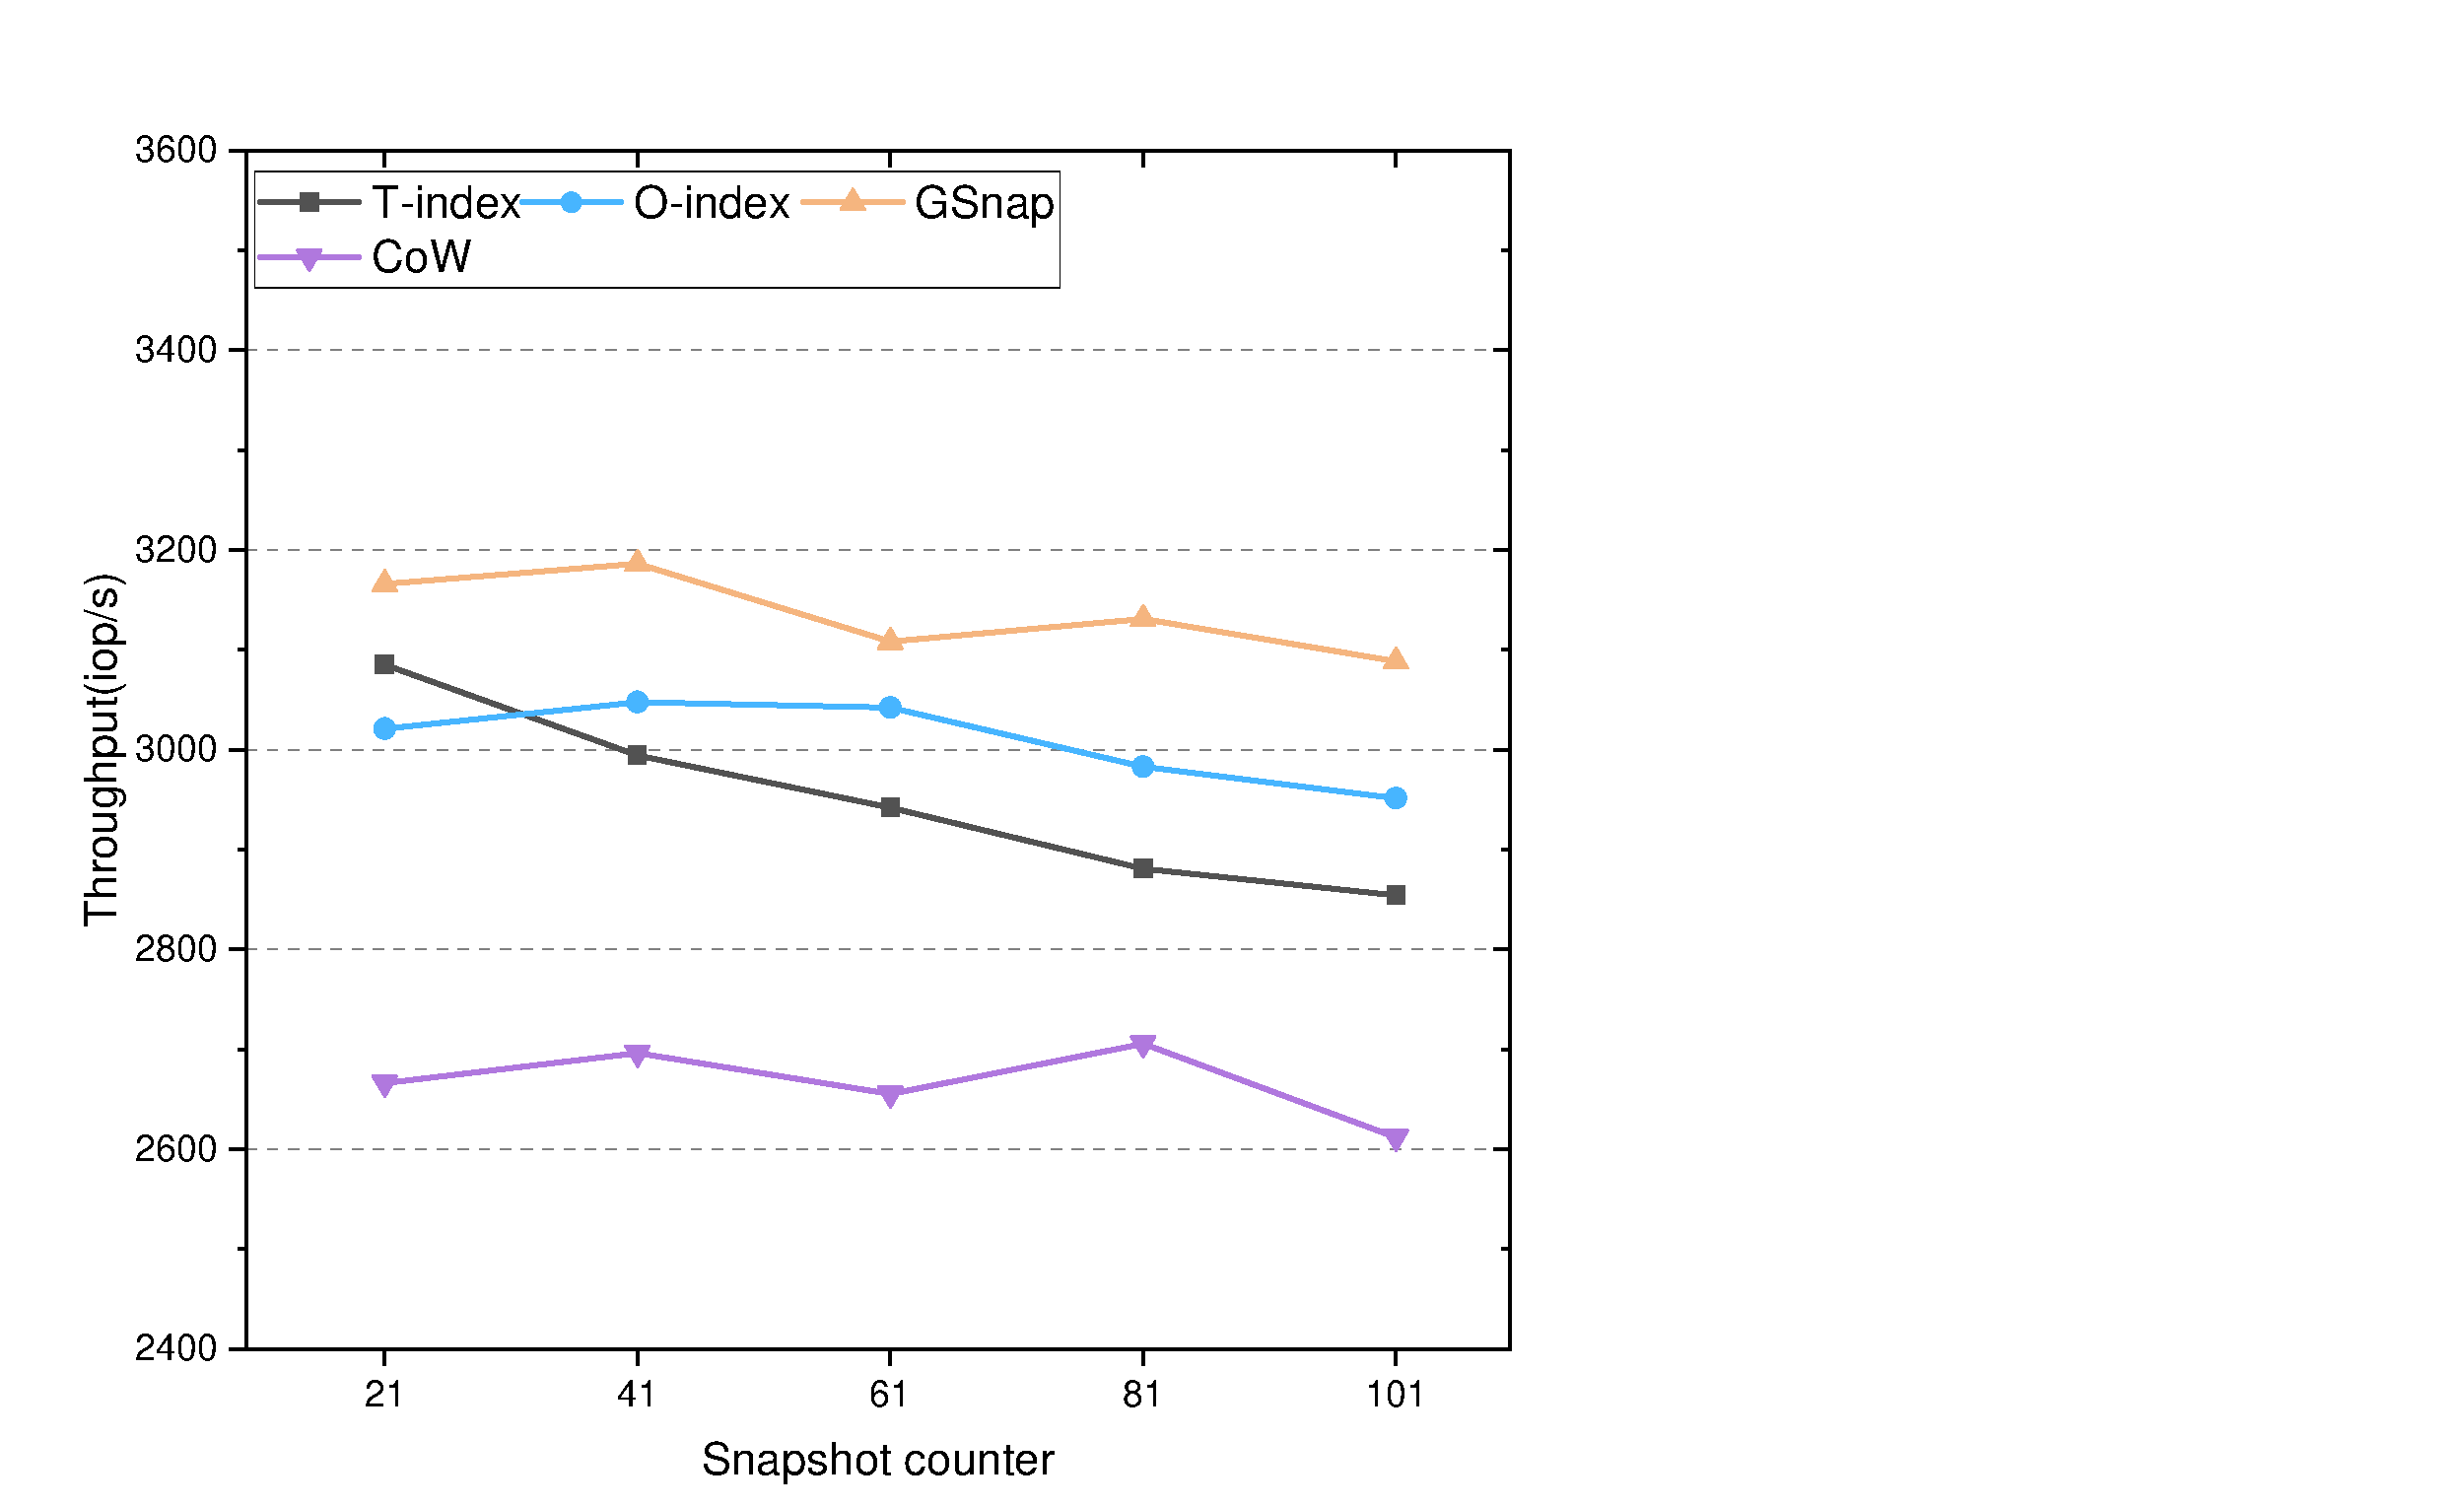
\includegraphics[width=6cm]{figures/ceph_pic/eval_balanced.pdf}
		\label{banlanced}}
	\hspace{-5in}
	\subfigure[Read-Only]{
		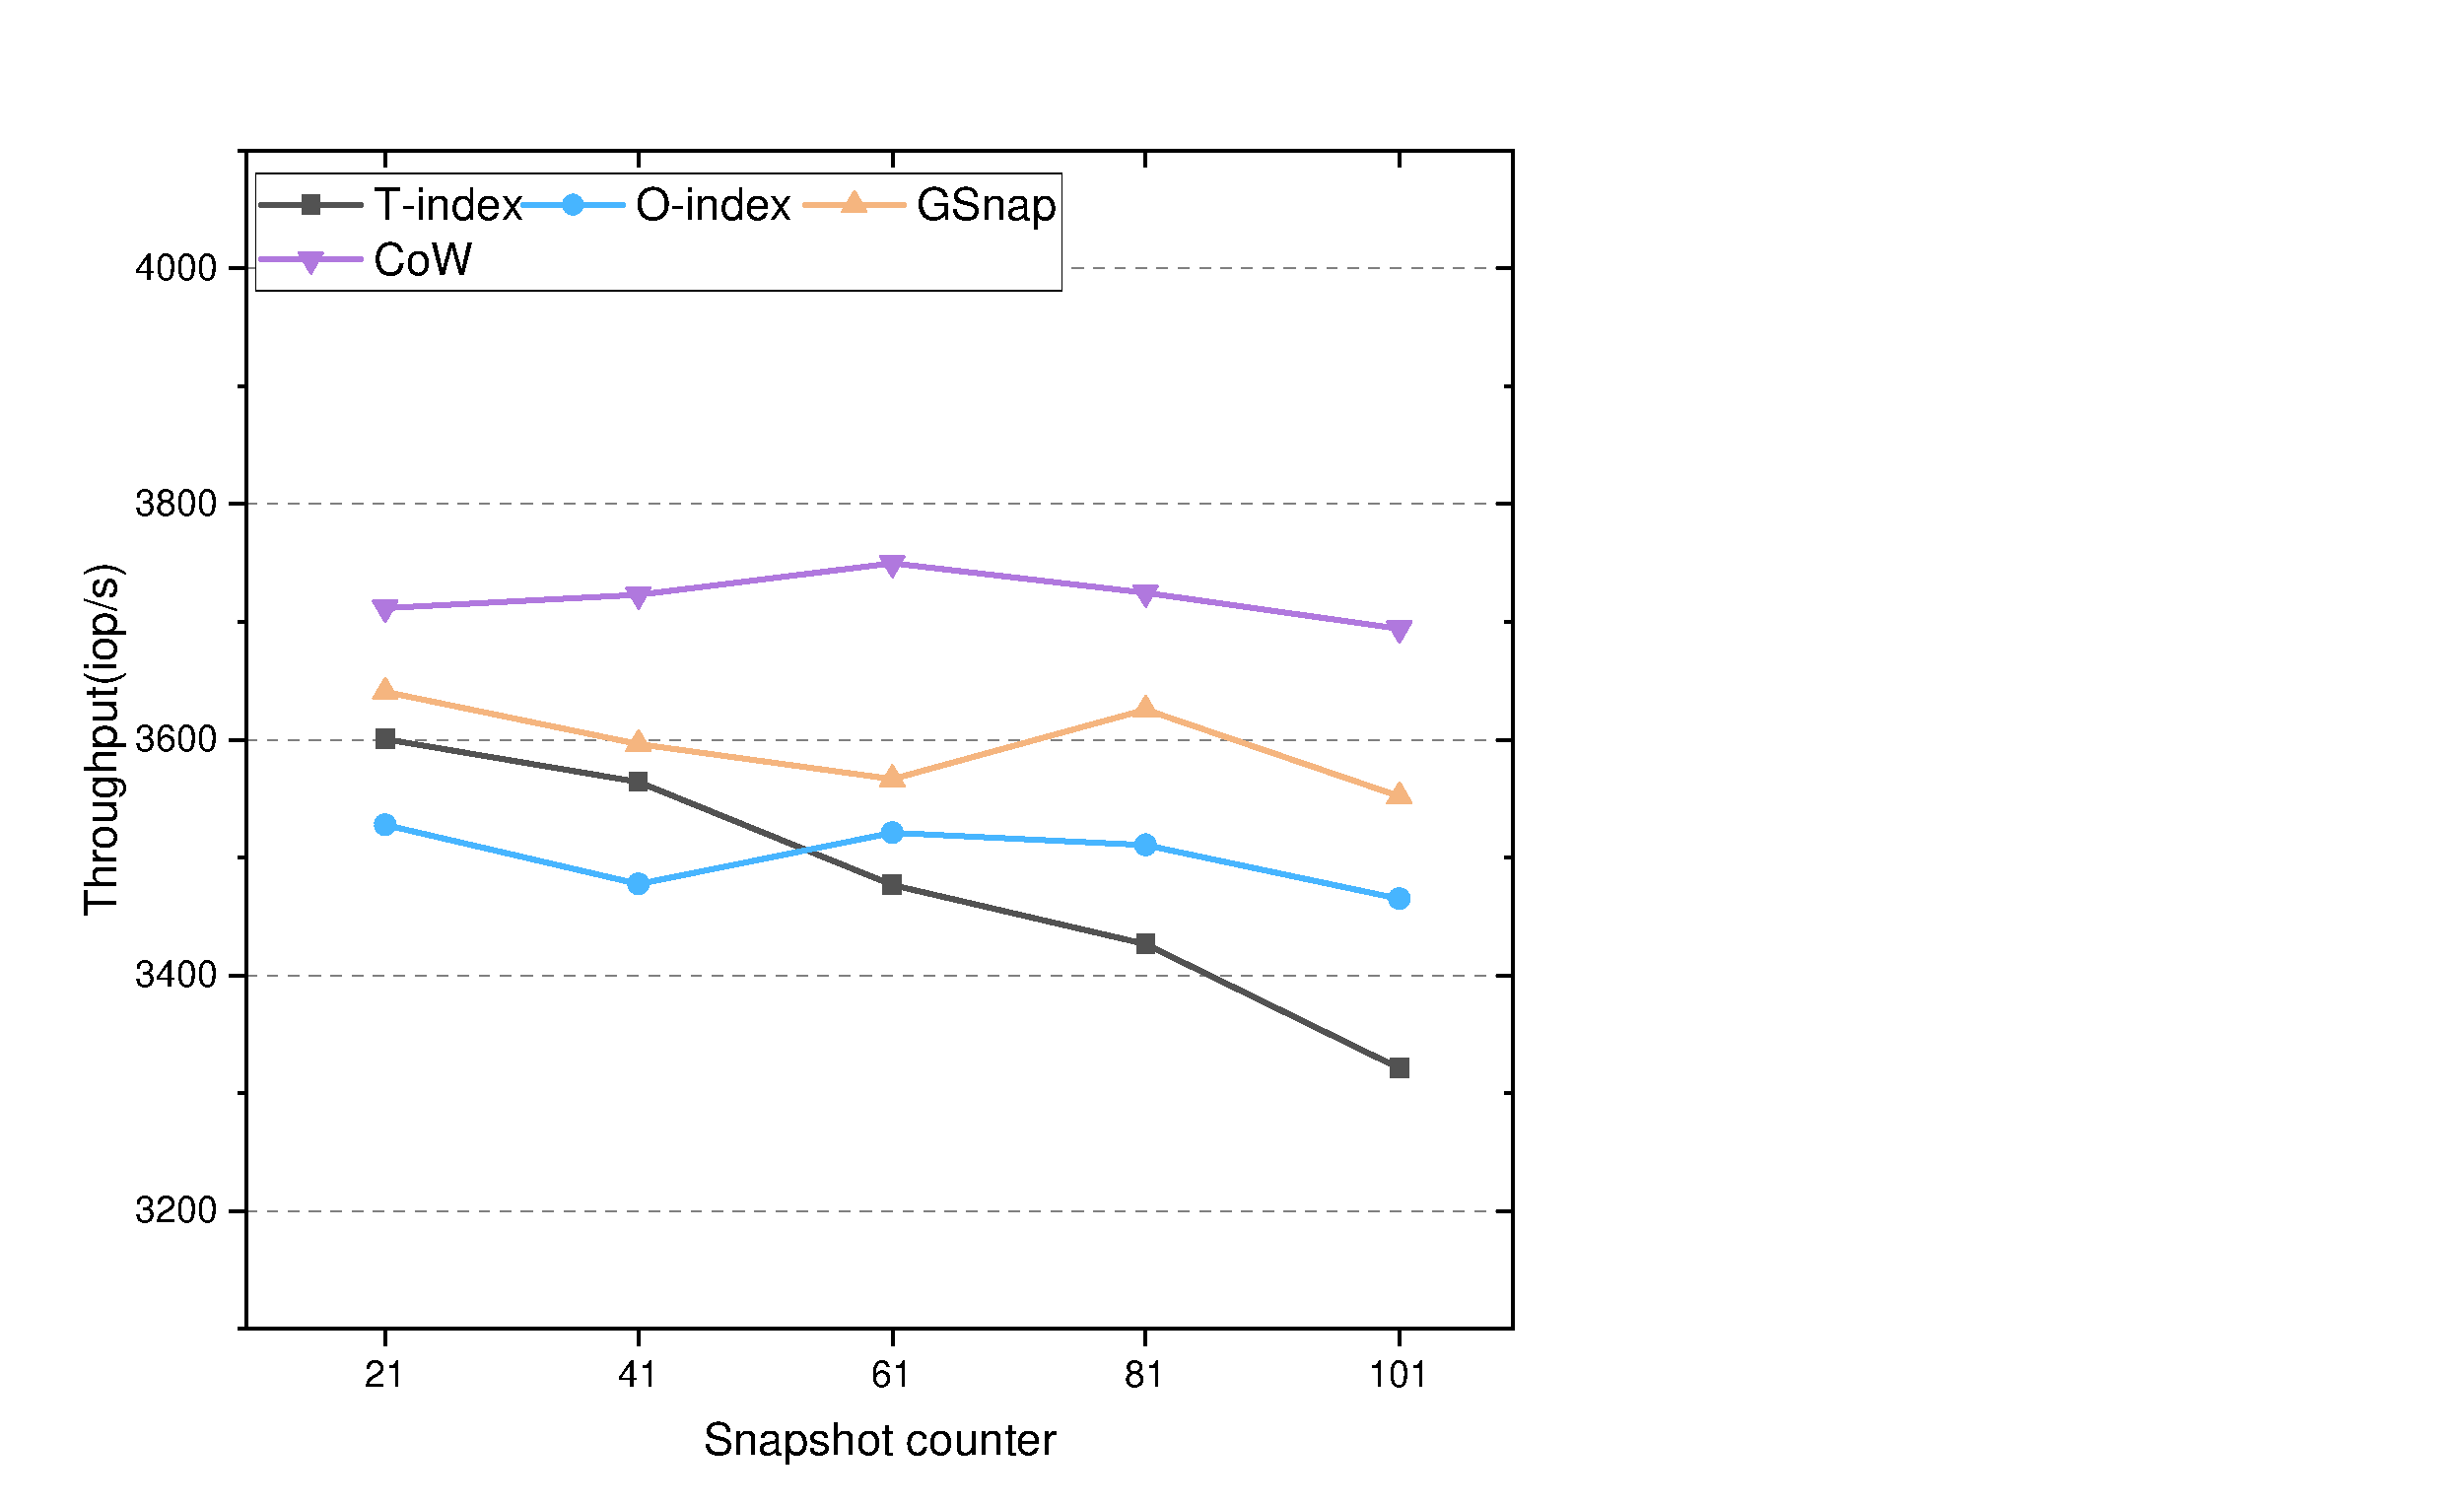
\includegraphics[width=6cm]{figures/ceph_pic/eval_read.pdf}
		\label{write-only}}
	\vspace{-0.3cm}
	\caption{The I/O performance for GSnap}
	\label{fig:IO_performance}
	\vspace{-0.2cm}
\end{figure*}


\label{IPerforamce}
We also evaluate the I/O performance in the XFS and compare the
throughput under various number of snapshot, highlighting the impact
of indexes on locating data blocks. Specifically, the read/write ratio
set as: read-only, balanced (50\% read / 50\% write) and
write-only. the block size is default set to 4MB.

As shown in Figure \ref{fig:IO_performance}, the performance of gsnap
is stable as the number of snapshots increases. The reason is that the
group cuts off the dependency of snapshots. When locating data blocks,
only the snapshots in the group need to be accessed. Even if O-index
only needs to access the previous snapshot, it copies all leaf
nodes. Of course, the performance of the first snapshot in the group
is lower than O-index since it accesses the prior group and constructs
a complete index. In read-only workloads, CoW performs better than
other indexes because only the current snapshot needs to be
accessed. As the write ratio increases, the performance degrades
significantly due to the double write.  The performance of T-index
decreases as the number of snapshots increases in read-only
workloads. Because it needs to access indexes iteratively when looking
for data blocks. As shown in Figure \ref{write-only}, the iterative
traversal of data blocks is reduced in the write-only workload, the
performance is still degraded. The reason is that the lazy eviction of
the previous indexes leads cache overhead increase.

\section{Related work}
\label{Relatedwork}
\textbf{Snapshot Technologies.}  Snapshot Implementations such as:
CoW, CoW with background copy (CoW+), Split Mirror Redundant Array of
Independent Disks (SMRAID), Continuous Data Protection (CDP)
\cite{garimella2006understanding}, RoW. The snapshot technologies have
been extensively compared and analysed
\cite{mahipal2021virtual,joseph2019securing,almulla2013distributed,subramanian2014snapshots}. CDP
is made incrementally and used in synchronous data mirroring and
Incremental Snapshot adapts a timestamp-based incremental approach
with rollback provisioning. In summary, the write overhead of CoW,
CoW+, SMRAID are suffered by their methodologies, their derivative
technologies induce overheads for regular I/O and dramatic increase of
sync operations when snapshots are present
\cite{subramanian2014snapshots,li2012irow}.
%Incremental Snapshot and CDP are mostly dependent on the underlying technology used for taking snapshots and network bandwidth.
Traversing to locate data blocks can cause performance degradation
because fragmentation increases as snapshots increase.  Amazon EBS
\cite{varia2014overview} has an optimized RoW snapshot index that
stores the regions which are continuous unchanged data blocks. The
region points to the last changed snapshot instead of the previous
snapshot to avoid iterative queries.  However, when the number of
snapshots grows, the size of each region shrinks and the number of
regions grows, considerably increasing the memory footprint of
indexes.

\textbf{Index Structure.}  \cite{DBLP:conf/icpads/LiZCY14} uses the
bitmap method to record the block number, but in the RoW, the
dependency relationship still exists between the snapshots, and there
is an iterative traversal to find the data
block. \cite{tsikoudis2018rql,shrira2005snap,tsikoudis2020rid} use a
log structure to record snapshot metadata, and the metadata updating
overhead of log structure is heavy when snapshots are continuously
added and deleted. Parallax \cite{DBLP:conf/eurosys/MeyerACLFHW08}
leverages a tree structure to maintain snapshot indexes, and adopt
ratix tree to reduce leaf nodes overhead. We also adopt the ratix tree
structure and borrow the ZFS \cite{rodeh2003zfs} to share child nodes
between trees to reduce indexing overhead. Amazon EBS
\cite{varia2014overview} optimizes the structure of the leaf node on
the optimized index, setting fixed-length leaf nodes to store
continuous unmodified data blocks to reduce the memory consumption of
the index. However, the leaf node locating becomes complicated and the
overhead of index updating increases when the snapshot is
updated. Moreover, as the write ratio increases, the index degenerates
the optimized index. Therefore, it is not applicable for the scenario
of accessing a large number of snapshots.

\textbf{Snapshot Implementation Layers.}  In the database layer,
database administrators can choose mysqldump \cite{mysqldump} for
logical backup and Percona Xtrabackup \cite{xtrabackup} for physical
backup. A logical backup stores the queries executed by transactions,
while the physical backup copies the raw data to storage. In the
recovery process, the stored queries are re-executed, or backup data
are copied to a database directory. However, recovery operations in
the existing tools take a long time, since these recovery procedures
involve a large amount of I/O operations induced by database queries
or raw data copies.  Snapshots techniques supported by file systems
and the block layer can be adopted for the backup and recovery of
database. Network Appliance NAS filers, the Sun ZFS
\cite{rodeh2003zfs} and BTRFS \cite{rodeh2013btrfs} organize the file
as a tree with data at the leaf level and meta-data maintained in
internal nodes.
%Each snapshot consists of a separate tree, but snapshot may share
%subtrees with other snapshots.  Though creating a snapshot is
%lightweight, the overhead of first write to a block is heavy once a
%snapshot is created because the entire tree of meta-data nodes needs
%to be copied and linked to the root node of the snapshot.
LVM \cite{hasenstein2001logical} operates the storage device and
provides fast snapshot creation and restoration using CoW. However,
the CoW negatively affects run-time performance since it performs
redundant writes due to data copies.

\section{conclusions}
\label{Conclusions}
In this paper, we propose GSnap, a lightweight RoW-based snapshot
index for large-scale backup and fast recovery. It performs a hybrid
design to split the dependency of snapshot indexes in a
group. In-group snapshot indexes reduce memory overhead by sharing
subtrees. The index can directly locate data blocks instead of
iterative traversal. Loading target snapshot group indexes instead of
indexes dependent, which balances index memory and recovery time
overhead.  The experimental results show that GSnap achieves higher
performance than compared indexes.









\bibliographystyle{ACM-Reference-Format}
\bibliography{sample-base}


%%
%% If your work has an appendix, this is the place to put it.
%\appendix



\end{document}
\endinput
%%
%% End of file `sample-xelatex.tex'.
